%------------------------------------------------------------
% Description : Теория меры
% Author      : Iliya Tikhonenko <iliya.t@mail.ru>
% Created at  : Tue Feb 21 00:00:16 MSK 2017
%------------------------------------------------------------
\documentclass[draft, timbord]{longnotes}
\usepackage{tmath}
\usepackage{cussymb}
\usepackage{silence}
% \WarningFilter{latex}{Reference}
\graphicspath{{../../img/}}
\begin{document}
\paragraph{Системы множеств}
\label{par:meas::setsys}

\begin{defn}\label{defn:meas::setsys::sub}
  Пусть здесь (и дальше) $X$~--- произвольное множество. Тогда $\pset(X) \equiv 2^X$~--- множество
  всех подмножеств $X$.
\end{defn}
\begin{exmp*}
  $X = \{1 \intrng n\} \Rightarrow \# \pset (X) = 2^n$ (это количество элементов, если что)
\end{exmp*}

\begin{defn}[Алгебра]\label{defn:meas::setsys::alg}
  Пусть $\alg \subset \pset (X)$. Тогда $\alg$~--- алгебра множеств, если
  \begin{enumerate}
    \item $\varnothing \in \alg$
    \item $X \in \alg$
    \item $A,B\in \alg \Rightarrow A \cap B, A \cup B, A \setminus B \in \alg$
  \end{enumerate}
\end{defn}
\begin{rem*}
  Заметим, что в алгебре пересечение (или объединение) \emph{конечного} числа её элементов лежит в
  алгебре.  Это можно доказать простой индукцией. А вот для бесконечных объединений пользоваться
  индукцией уже нельзя, ведь $\infty \not\in \N$. 
\end{rem*}

\begin{defn}[$ \sigma $-алгбера]\label{defn:meas::setsys::sigalg}
  Пусть $\alg \in \pset(X)$. Тогда $\alg$~--- $ \sigma $-алгебра, если 
  \begin{enumerate}
    \item $\alg$~--- алгебра
    \item $A_1, \dotsc, A_n \in \alg \Rightarrow \bigcup_{k=1}^ \infty A_k \in\alg, 
      \bigcap_{k=1}^{ \infty } A_k \in \alg $
  \end{enumerate}     
\end{defn}

\begin{defn}\label{defn:meas::setsys::sigshell}
  Пусть $\mathcal E \subset \pset(X)$. Тогда 
  \[
  \sigma(\mathcal E) := \bigcap\,\{\alg \mid \alg\text{~--- $\sigma$-алгебра, $\alg \supset
  \mathcal E $}\}
  \]
  эта конструкция~--- сигма-алгебра, просто аксиомы проверить.
\end{defn}

\paragraph{Борелевская сигма-алгебра}
\begin{defn}\label{defn:meas::setsys::borel}
  Пусть $\open$~--- все открытые множества в $\R^n$. Тогда $\mathpzc B_n = \sigma(\open)
  $~--- борелевская $\sigma$-алгебра в $\R^n$.
\end{defn}

\begin{defn}[Ячейка в $\R^n$ ]\label{defn:meas::setsys::cell}
  Обозначать её будем $\Delta^n$, по размерности соответствующего пространства.
  \[
    \Delta^1 = \begin{cases}
      [a;b) \\
      (-\infty;b) \\
      [a;+\infty) \\
      (-\infty;+\infty)
    \end{cases} \quad
    \forall\, n \;\: \Delta = \prod_{k=1}^n \Delta^1 _k 
  \]
  Ещё введём алгебру $\alg = \Cell_n = \{ A \mid A = \bigcup_{k=1}^p \Delta_k\}$
\end{defn} 

\begin{lem}\label{lem:meas::setsys::algsubset}
  Пусть $\mathcal E_1, \mathcal E_2 \subset \pset(X)$, $\sigma(\mathcal E_1) \supset \mathcal E_2$.
  Тогда $\sigma(\mathcal E_1) \supset \sigma(\mathcal E_2)$
\end{lem}
\begin{lproof}
  $\sigma(.)$ от обеих частей.
\end{lproof}
\begin{thrm}\label{thrm:meas::setsys::borelcell}
  $\borel_n = \sigma(\Cell_n)$.
\end{thrm}
\begin{tproof}
  \begin{description}
    \item[$\sigma (\open) \supset \Cell$] Покроем открытыми квадратиками.
    \item[$\sigma (\Cell) \supset \open$] Для упрощения жизни $\open \supset G \in \R^2$.
      Рассмотрим классы ячеек
      \[
        \mathcal C_k = \left\{
          \left[\frac m 2; \frac{m+1}{2^k}\right) 
          \times 
          \left[\frac n 2; \frac{n+1}{2^k}\right) \subset G
          \:\middle|\: m,n \in \Z
        \right\}
      \]
      Осталось показать, что любую точку из $G$ покрывает ячейка какого-то класса.
      
      Каждая точка открытого множества входит с какой-то окрестностью, которую можно считать
      обединением множеств из базы топологии. Короче, есть маленький открытый квадратик, 
      содержащий точку. 

      Так что теперь можно думать просто про одномерье.
      Ясно, что \[
        \exists\, m, k \that 
        \begin{cases}
          x-\varepsilon < \frac{m}{2^k} < x \\
          x+ \varepsilon >  \frac{m+1}{2^k} > x \\
        \end{cases}
      \]
      Для этого хватит, чтобы $ |x-\varepsilon ; x| > \frac{1}{2^k}$, например.
  \end{description}
\end{tproof}

\begin{exmp}\label{exmp:meas::setsys::borel}
%   \everymath{\displaystyle}
  Все множества нижё~--- борелевские.
  \begin{enumerate}[$\langle$1$\rangle$]
    \item $\open $.
    \item $\closed =\{A \mid \ov-{A} \in \open \}$.
    \item $\Biggl(A 
      = \bigcap_{\substack{{k=1}\\[0.12em]\mathclap{ G_k \in \open}}}^\infty G_k \Biggr)\in G_\delta$.
    \item $\Biggl(B 
      = \bigcup_{\substack{{k=1}\\[0.12em]\mathclap{ F_k \in \closed}}}^\infty F_k \Biggr)\in
      F_\sigma$.
    \item $\Biggl(C 
      = \bigcup_{\substack{{k=1}\\[0.12em]\mathclap{ A_k \in G_{\delta}}}}^\infty A_k \Biggr)
      \in G_{\delta\sigma}$.
  \end{enumerate}
  У всех этих множеств со сложными индексами $\delta$~--- пересечение, $\sigma$~--- объединение,
  $G$~--- операция над открытыми в самом начале, $F$~--- над замкнутыми.
\end{exmp}

\paragraph{Мера}
\label{par:meas::meas}

\begin{defn}\label{defn:meas::meas}
  Пусть задано $X$, $\alg \subset \pset (X)$, $A_k \in \alg$. Тогда $\mu \colon \alg \to [0;
  +\infty]$~--- мера, если 
  \begin{enumerate}
    \item $\mu(\varnothing) = 0$
    \item $\displaystyle\mu\Biggl(\underbrace{\bigsqcup_{k=1}^\infty A_k}_{\in \alg}\Biggr)
      = \sum_{k=1}^\infty \mu(A_k)$. Здесь никто не обещает, что будет именно $\sigma$-алгебра.
  \end{enumerate}
  Множества $A \in \alg$ в таком случае называются $\mu$-измеримыми.
\end{defn}

\begin{exmp}\label{exmp:meas::meas::delta}
  $a \in X$, $\displaystyle\mu(A) = \begin{cases}
    1, & a\in A \\
    0, & a \not\in A
  \end{cases}$ ~--- $\delta$-мера Дирака.
\end{exmp}
\begin{exmp}\label{exmp:meas::meas::mol}
  $a_k \in x$, $m_k \geqslant 0$, $\displaystyle\mu(a) 
  := \sum_{\mathclap {k\colon a_k \in a}} m_k$~---
  <<молекулярная>> мера.
\end{exmp}

\begin{exmp}\label{exmp:meas::meas::cnt}
  $\mu(A) = \# A$~--- считающая мера. \note{она считает, не считывает $\ddot\smile$}
\end{exmp}

\paragraph{Свойства меmы}

Здесь всюду будем рассматривать тройку $(X, \alg \subset \pset (X), \mu)$

\begin{prop}[Монотонность меры]\label{prop:meas::meas::monot}
  Пусть $A,B \in \alg$, $A \subset B$. \par Тогда $\mu(A) \leqslant \mu(B)$.
\end{prop}
\begin{lproof}
  $B = A \sqcup C$. Дальше очевидно
\end{lproof}
\begin{prop}\label{prop:meas::meas::diff}
  Пусть $A,B \in \alg$, $A \subset B$, $\mu(B) < +\infty$.  \par 
  Тогда $ \mu(B\setminus A) = \mu(B) - \mu(A)$.
\end{prop}
Мемы $A,B$ конечны, иначе нельзя вычитать.
\begin{prop}[Усиленная монотонность]\label{prop:meas::meas::enfmont}
  Пусть $A_{1 \intrng n}, B \in \alg$, $\bigsqcup_i A_i \subset B$ . \par
  Тогда $\displaystyle\sum_{k=1}^n \mu(A_k) \leqslant \mu B$
\end{prop}
\begin{rem}\label{rem:meas::meas::enfmont}
  Можно усилить и на случай $n = \infty$, предел есть, так как члены возрастают.
\end{rem}

\begin{prop}[Полуаддитивность меры]\label{prop:meas::meas::semiadd}
  Пусть $B_{1 \intrng n}, A \in \alg$, $A \subset \displaystyle \bigcup_{k=1}^n B_k$. \par
  Тогда $\displaystyle\mu A \leqslant \sum_{k=1}^n \mu(B_k)$.
\end{prop}
\begin{lproof}
  Сделать $B_k$ дизъюнктными: $C_k = B_k \setminus \bigcup_{j <k} B_k$. Затем представить $A$ как
  дизъюнктное объединение $D_k \colon D_k = C_k \cap A$. Так можно сделать, потому что
  \[
    A = A \cap \bigcup_{k=1}^n B_k = A \cap \bigsqcup_{k=1}^n C_k = \bigsqcup_{k=1}^n A \cap C_k
  \]
  Ну а тогда
  \[
    \mu (A) = \sum_k \mu D_k \leqslant \sum_k \mu C_k \leqslant \sum_k \mu B_k
  \]
\end{lproof}


\begin{prop}[Непрерывность меры снизу]\label{prop:meas::meas::bcont}
  Пусть $A_1 \subset A_2 \subset \cdots$, $A_k \in \alg$,
  $\left(\displaystyle A = \bigcup_{k=1}^\infty A_k\right) \in \alg$.
  \note{Опять-таки никто не сказал, что $\alg$~--- $\sigma$-алгебра.} \par
  Тогда $\displaystyle \mu A = \lim_{n\to \infty} \mu A_n$
\end{prop}
\begin{lproof}
  Строим разности $C_k = A_{k+1} \setminus A_k$,$C_0 = A_1$ а $A= \bigsqcup_k C_k$.
  
  Вот ещё картинка: \ref{fig:meas::meas::eudoks}, для пущей очевидности.

   \begin{figure}
   \begin{center}
     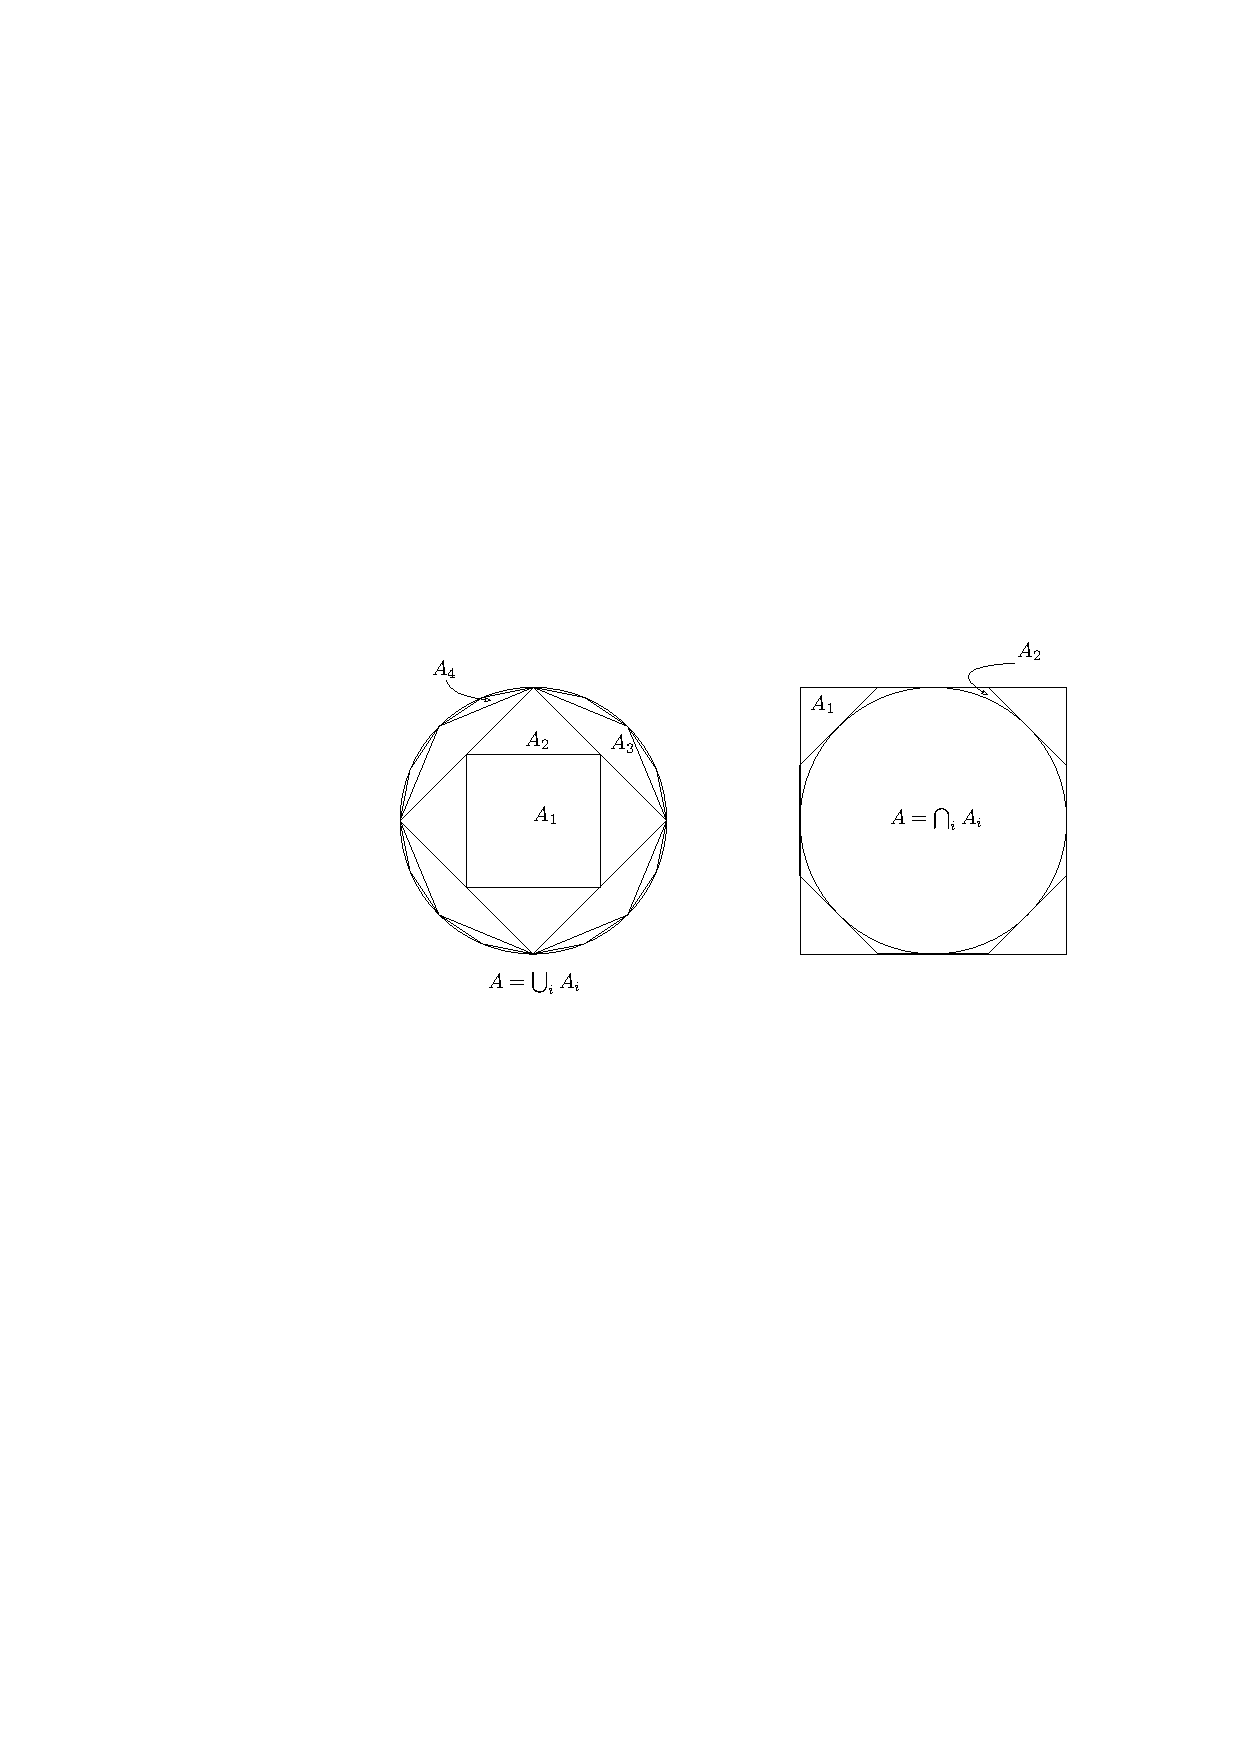
\includegraphics[scale=1]{meas/eudoks}
   \end{center}
   \caption{Метод исчерпывания Евдокса}
   \label{fig:meas::meas::eudoks}
   \end{figure}
   
\end{lproof}
\begin{prop}[Непрерывность меры сверху]\label{prop:meas::meas::ucont}
  Пусть $A_1 \supset A_2 \supset \cdots$, $A_k \in \alg$, 
  $\displaystyle A = \bigcap_{k=1}^\infty A_k \in \alg$, $\mu A_1 < +\infty $.
  \par
  Тогда $\displaystyle \mu A = \lim_{n\to \infty} \mu A_n$
\end{prop}
\begin{lproof}
  Сначала заметим, что все меры сделаны конечными, ведь нужно считать разности мер, а
  это так себе.

  Снова сделаем разности $C_k = A_k \setminus A_{k+1}$
  \[
    \bigsqcup_{k=1}^n  C_k = A_1 \setminus A_{n+1} 
    \Rightarrow \mu (A_{n+1}) = \mu (A_1) - \mu \left( \bigsqcup_{k=1}^n  C_k \right)
  \]
  Понятно, что \[
    \lim_{n\to \infty} \bigsqcup_{k=1}^n  C_k \sqcup A = \bigsqcup_{k=1}^\infty  C_k \sqcup A = A_1
  \]
  Так что \[
    \lim_{n\to \infty} \mu \left( \bigsqcup_{k=1}^n  C_k \right) = \mu (A_1) - \mu (B)
  \]
  Но тогда\[
    \lim_{n\to \infty } \mu (A_n) = \lim_{n\to \infty } \mu (A_{n+1}) = \mu B
  \]
\end{lproof}


\begin{defn}\label{defn:meas::ledeg::compl}
  Пусть задана тройка $(X, \alg_\sigma, \mu)$. Тогда $\mu$~--- полная, если 
  \[
    \forall\,A \in \alg : \mu A = 0 \;\: \forall\, B \subset A, B \in \alg \holds \mu B = 0
  \]
\end{defn}

\begin{defn}\label{defn:meas::ledeg::sfin}
  Мера $\mu$  на $\alg$ называется $\sigma$-конечной, если 
  \[
    \exists\, X_n \in \alg, \mu X_n < + \infty \that \bigcup_{n=1}^\infty X_n = X
  \]
\end{defn}

\begin{defn}\label{defn:meas::ledeg::mcont}
  Пусть $\alg_1, \alg_2$~--- сигма-алгебры подмножеств $X$, $\alg_1 \subset \alg_2$,
  $\mu_1 \colon \alg_1 \to [0;+\infty] $, $\mu_2 \colon \alg_2 \to [0;+\infty]$. 
  Тогда $\mu_2$ называется продолжением $\mu_1$.
\end{defn}

\begin{thrm}[Лебега-Каратеодора]\label{thrm:meas::ledeg::dist}
  Пусть $\mu$~--- сигма-конечная мера на $\alg$. Тогда
  \begin{enumerate}
    \item Существуют её полные сигма-конечные продожения
    \item Среди них есть наименьшее: $\ov-\mu$. 
      Её ещё называют стандартным продолжением.
  \end{enumerate}
\end{thrm}

\begin{defn}[Внешняя мема]\label{defn:meas::ledeg::exter}
  Пусть $E \subset X$. Положим
  \[
    \mu^* (E) := \inf \left\{ \sum_{k=1}^\infty \mu A_k \: 
    \middle|\; A_k \in \alg, E \subset \bigcup_{k=1}^\infty A_k \right\}
  \]
  Тогда $\mu ^* $~--- внешняя мема, порождённая $\mu$. Она не мера.
\end{defn}

\begin{exmp}
  Например, сигма-алгебра из вертикальных полос на квадратике. Аддитивность сломается, если
  взять 2 непересекающихся горизонтальных <<лоскутка>> один по другим.
\end{exmp}

Так, вот про идею доказательства. 
Внешняя мема~--- очень привлекательная вещь, но не мера. 

Давайте разрешим лишь определённый набор множеств. Назовём их хорошо разбивающими.

\begin{defn}\label{defn:meas::ledeg::wellspl}
  Пусть $E \subset A$. Тогда $E$~--- хорошо разбивающее, если \[
    \forall\, A \in \alg \holds \mu A = \mu^* (A \cap E) + \mu ^* (A \setminus E)
  \]
\end{defn}

Хорошо разбивающие явно содержат исходную алгебру.

Для тех же вертикальных полос в хорошо разбивающие попадут все 
множества, проектирующиеся в точку на ось $\perp$ полосками.

\paragraph{Объём в \texorpdfstring{$\R^n$}{R\^{}n}. Мера Лебега }
\label{par:meas::lebeg}

\begin{defn}\label{defn:meas::lebeg::cell}
  Пусть $\Delta = \Delta_1 \times \dotsm \times \Delta_n$, $\Delta_k = [a_k, b_k)$.
  Тогда
  \[
    \begin{split}
      v_1 \Delta_k \equiv | \Delta_k| &:= \begin{cases}
        b_k - a_k, & a_k \in \R \land b_k \in \R \\
        \infty, & \text{иначе}
      \end{cases} \\ 
      v \Delta \overset{(\in R^n)}\equiv v_n \Delta &:= |\Delta_1| \dotsm |\Delta_n|
    \end{split}
  \]
  Для всего, что $\in \Cell_n$, представим его в виде дизъюнктного объединения $\Delta_j$.
  Тогда $vA := \sum_{j=1}^q v \Delta_j $.
\end{defn}

\begin{rem*}
  Здесь радикально всё равно, входят ли концы~--- у них мера ноль. 
\end{rem*}

\begin{thrm}\label{thrm:meas::ledeg::finadd}
  $v$~--- конечно-аддитивен, то есть \[
    \forall\, A, A_{1 \intrng p} \in \Cell\, , A = \bigsqcup_{k=1}^p A_k
    \:\; \holds  vA = \sum_{k=1}^p v A_k
  \]
\end{thrm}
\begin{tproof}
  На клеточки побить.
\end{tproof}

\begin{thrm}\label{thrm:meas::ledeg::infadd}
  $v$~--- счётно-аддитивен, то есть \[
    \forall\, A, A_{1 \intrng } \in \Cell\, , A = \bigsqcup_{k=1}^\infty  A_k
    \:\; \holds  vA = \sum_{k=1}^ \infty  v A_k
  \]
\end{thrm}
Сначала докажем маленькую лемму.
\begin{lem}\label{lem:meas::ledeg::openclcell}
  Пусть $\Delta$~--- ограниченная ячейка в $\R^n$. Тогда 
  \[
    \exists\, \Delta' \in \open, \Delta'' \in \closed 
    \that 
    \left\{
      \begin{aligned}
        v \Delta'  &< v \Delta + \varepsilon  \\
        v \Delta'' &> v \Delta - \varepsilon 
      \end{aligned}
    \right.
  \]
\end{lem}
\begin{lproof}
  Например, для $\Delta = \prod_k [a_k; b_k)$ \[
    \begin{split}
      \Delta_i'  &= \prod_{k=1}^n \left(a_k-\frac 1 i ; b_k\right) \\
      \Delta_i'' &= \prod_{k=1}^n \left[a_k ; b_k - \frac 1 i\right] \\
    \end{split}
  \]
  Увеличивая $i$ можно добраться до любого $\varepsilon$.
\end{lproof}
\begin{tproof}[Счётной аддитивности объема]
  Здесь в конспекте лишь частный случай про ячейки. 
  А по-хорошему $\Cell$ содержит и любые конечные объединения ячеек.
  Утверждается, что там тоже самое, только возни сильно больше.

  Пусть $A = \Delta$, $A_k = \Delta_k$, причём они все конечны.
  Рассмотрим
  \begin{align*}
    \Delta_k' \supset \Delta &\that v \Delta_k' < v \Delta_k + \frac{\varepsilon}{2^k},\\
    \Delta'' \subset \Delta    &\that v \Delta'' > v \Delta - \varepsilon ,
  \end{align*}
  штрихи имеют смысл как в лемме.

  Тогда\[
    \Delta''  \subset \bigcup_{k=1}^\infty \Delta_k ' 
  \]

  По определению компактности, \[
    \exists\, (l_k) \that \Delta'  \subset \bigcup_{l=1}^N \Delta_{k_l}''
  \]
  
  Так что из счётной аддитивности
  \[
    v \Delta'' \leqslant v \left(\bigcup_{l=1}^N \Delta_{k_l}'\right)
    = \sum_{l=1}^N v \Delta_{k_l}' < \sum_{l=1}^N v \Delta_{k_l} + \varepsilon
  \]
  А \[
    \sum_{l=1}^N v \Delta_{k_l} <  \sum_{k=1}^\infty v \Delta_{k}
  \]
  Так что 
  \[
    v \Delta < \sum_{k=1}^\infty v \Delta_{k} + 2\varepsilon \Rightarrow
    v \Delta \leqslant \sum_{k=1}^\infty v \Delta_{k} 
  \]

  В другую сторону не так понятно. Для частных сумм из конечной аддитивности
  \[
    \forall\, N \holds \sum _{k=1}^N v \Delta_k \leqslant v \Delta
  \]
  При увеличении $N$ сумма лишь возрастает, но она и ограничена. Значит предел есть.
  Тогда $\sum_k v \Delta_k \leqslant v \Delta$.
\end{tproof}



\begin{defn}[Мера Лебега]\label{defn:meas::ledeg::lebeg}
  $X=\R^n$, $\alg= \Cell_n$. Тогда $\lambda_n = \ov-{v_n}$, $\mathpzc M = \ov-{\alg}$~--- мера
  Лебега и алгебра множеств, измеримых по Лебегу, соответственно.
\end{defn}

\subparagraph{Свойства меры Лебега}

\begin{enumerate}[(1) $\triangleright$]
  \item $\lambda \{x\} = 0$
  \item $\lambda \bigl(\{x_k\}_{k}\bigr) = 0$
  \item $\borel \subset \lebesgue$. Это, кстати, не очевидно. С другой стороны, для них
    есть покрытие квадратиками.
  \item $L \subset \R^m, m<n \Rightarrow \lambda_n L  = 0$
\end{enumerate}

А это уже целая теормема.
\begin{thrm}[Регулярность меры Лебега]\label{thrm:meas::ledeg::reg}
  Пусть $A \in \lebesgue$, $\varepsilon > 0$. Тогда 
  \[
    \exists\, G \in \open, F \in \closed \that F \subset A \subset G \land 
    \begin{cases}
      \lambda(G \setminus A) < \varepsilon \\
      \lambda(A \setminus F) < \varepsilon 
    \end{cases}
  \]
\end{thrm}
\begin{tproof}
  \begin{enumerate}[(1)]
    \item Сначала разберёмся с конечными множествами. Из определения инфимума, 
      $\exists\, \{\Delta_k\} \that \lambda(A) > \sum_k \Delta_k - \frac{\varepsilon}{2} $.

      Снова подберём $\Delta'_k$, как в \ref{thrm:meas::ledeg::infadd},
      только $\ov~\varepsilon = \frac{\varepsilon}{2^{k+1}}$.
      В таком случае \[
        \lambda(A) > \sum_k \Delta_k - \varepsilon / 2 > \sum_k \Delta_k ' - \varepsilon
      \]
    \item \underdev, но что-то жесть. Обычно доказывают что  $\lambda \inf G_k = \lambda A$.
  \end{enumerate}
  Кажется, победа. Для замкнутых можно доказывать все для $X \setminus A$ сводя к первому
  пунку. Как-то так\[
    (F^c \setminus A^c) = (F^c \cap A) = (A \cap F^c) = A \setminus F
  \]
\end{tproof}
\begin{cor}\label{cor:meas::ledeg::gdelta}
  $\forall\, A \; \exists\, D \in G_\delta \that A = D \cup N$, $\mu(N) = 0$.
\end{cor}

\begin{exmp}[Пример неизмеримого множества (по Лебегу)]\label{exmp:meas::ledeg::unmeasbl}
  Пусть $x \sim y \Leftrightarrow y-x \in \Q$ и всё это лежит на отрезке $I=[0;1]$.
  Пусть $R_k$~--- $k$-ый смежный класс по $\sim$. Тогда $S = \sqcup_k R_k$.
  
  \emph{Выберем} $E \colon \forall\, k \holds | E \cap R_k| = 1$. Как видно, $\{E_j\}$ отличаются
  сдвигом на $r \in \Q$. Будем считать, что сдвиг~--- это скорее поворот, как бы замыкаем
  начало и конец отрезка, так что $E_j + r \in I \;\: \forall\, k\in \Z, r\in[0;1]\cap \Q$.

  Тогда $I = \sqcup_k E_k$, $\forall\, j,k \holds\lambda E_j = \lambda E_l $.
  
  Но теперь
  \[
    1= \lambda I = \sum_{k=1}^\infty \lambda E_k = \sum_{k=1}^\infty a 
  \]
  А бесконечная сумма вещественных чисел либо $0$ либо $\infty$.
\end{exmp}

\paragraph{Измеримые функции}
\label{par:meas::mfun}

\begin{defn}\label{defn:meas::mfun}
  Пусть задана тройка $(X, \alg_\sigma, \mu)$. Пусть ещё $f\colon X \to \R$. Тогда 
  $f$ называется измеримой относительно $\alg$, если 
  \[
    \forall\, \Delta \subset \R, \text{$\Delta$~--- связно} \holds f^{-1} (\Delta) \in \alg
  \]
\end{defn}

\begin{thrm}\label{thrm:meas::mfun::diftyps}
  Пусть $f$ измеримо относительно $\alg$. Тогда измеримы и следующие (Лебеговы) множества
  \begin{description}
    \item[1 типа] $\{x \in X \mid f(x) < a\} \equiv X [f < a]$
    \item[2 типа] $\{x \in X \mid f(x) \leqslant a\} \equiv X [f \leqslant a]$
    \item[3 типа] $\{x \in X \mid f(x) > a\} \equiv X [f > a]$
    \item[4 типа] $\{x \in X \mid f(x) \geqslant a\} \equiv X [f \geqslant a]$
  \end{description}
  При этом верно и обратное: если измеримы множества какого-то одного типа, то
  $f$ измерима.
\end{thrm}
\begin{tproof}
  Просто представляем множества одного типа, как пересечение или дополнение множеств другого.
  Можно бесконечные, потому что здесь $\alg$~--- $\sigma$-алгебра.
\end{tproof}

\begin{thrm}\label{thrm:meas::mfun::sp}
  Пусть $f_1, \dotsc, f_n$ измеримы относительно $\alg$ и $g\colon \R^n \to \R$  
  непрерывна. Тогда измерима и $\varphi(x) = g(f_1(x), \dotsc, f_n(x))$.
\end{thrm}
\begin{tproof}
  Взять, например, $I = (-\infty, a)$. Он открыт, так что $g^{-1}(I) \in \open$.
  Из теоремы \ref{thrm:meas::setsys::borelcell} $G = \bigcup\limits_{k=1}^\infty \Delta _k$.
  А прообраз объединения~--- объединение прообразов. Так что $f^{-1} (G)$ измеримо.
\end{tproof}
\begin{rem*}
  В частности, $f_1 + f_2$ измерима.
\end{rem*}

\begin{thrm}\label{thrm:meas::mfun::lims}
  Пусть $f_1,f_2, \dotsc $ измеримы относительно $\alg$ .
  Тогда измеримы $\sup f_n, \inf f_n, \varliminf f_n, \varlimsup f_n, \lim f_n $.
  Последний, правда, может не существовать.
\end{thrm}
\begin{tproof}
  Например, для супремума. Он же по $n$, что
  \[
    X[ \sup f_n(x) < a ] = \bigcap_{n=1}^\infty X[f_n < a] 
  \]
  Каждое множество из пересечения $\in \alg$, значит и $\cap .. \in \alg$.
\end{tproof}

\begin{defn}\label{defn:meas::mfun::simp}
  Пусть $f \colon X \to \R$~--- измерима. Тогда она называется простой, если
  принимает конечное множество значений.
\end{defn}

\begin{defn}[Индикатор множества]\label{defn:meas::mfun::ind}
  \[
    E \subset X , \ind_E := \begin{cases}
      1, & x\in E \\
      0, & x\not\in E
    \end{cases}
  \]
  Он, как видно совсем простая функция.
\end{defn}
\begin{prop}\label{prop:meas::mfun::indmult}
  $\ind_{A \cap B} = \ind_A \cdot \ind_B$
\end{prop}
\begin{prop}\label{prop:meas::mfun::indsplitsum}
  Пусть $\sqcup_j A_j = A$, тогда $\sum_j \ind_{A_j} = \ind_A$.
\end{prop}

\begin{stat}\label{stat:meas::mfun::simpind}
  $f$~--- простая $ \Rightarrow f= \dsum_{k=1}^p c_k \ind_{E_k}$, $E_k$~--- дизъюнктны.
\end{stat}

\begin{thrm}\label{thrm:meas::mfun::simpseq}
  Пусть $f\colon X \to \R$, измерима, $f \geqslant 0$. Тогда 
  \[
    \exists\, (\varphi_n)\colon 0 \leqslant \varphi_1 \leqslant \varphi_2 \leqslant \cdots
    \that \varphi_n \nearrow f \text{ (поточечно)}
  \]
  Причём все $\varphi_i$~--- простые.
\end{thrm}

\begin{tproof}
  Зафиксируем какое-то $n$. Тогда
  \[
    [0; +\infty) = \bigsqcup_{k=0}^{n^2} \Delta_k, 
    \quad \Delta_k = \left[\frac{k}{n} , \frac{k+1}{n}\right), \; \Delta_{n^2} = [n; +\infty)
  \]
  Здесь мы порезали ось значений на $n^2$ интервалов. Выберем $e_k = f^{-1} (\Delta_k)$,
  $c_k = \min_{e_k}f(x) = \min \Delta_k = \frac{k}{n}$.

  Пусть $\psi_n = \dsum_{k=0}^{n^2} c_k \ind_{e_k}$.
  Тогда $\psi_n(x) \leqslant f(x) < \psi_k(x)+ \frac 1 n$. Видно, что поточечная сходимость есть.

  Теперь ещё обеспечим возрастание:
  \[
    \varphi_n = \max \{ \psi_1, \dotsc, \psi_n \}
  \]
\end{tproof}

\paragraph{Интеграл по мере}
\label{par:meas::int}

\begin{defn}\label{defn:meas::int}
  Пусть задана тройка $(X, \alg_\sigma, \mu)$, $f$~--- измерима.
\begin{enumerate}[{[1]}]
    \item $f$~--- простая. 
      \[
        \int _X f \, \del \mu := \sum_{k=1}^p c_k \mu E_k 
      \]
    \item $f \geqslant 0$.
      \[
        \int_X f \, \del \mu := \sup \Biggl\{ \int_X g \, \del \mu \:\Biggl|\: g\text{-простая},
          0 \leqslant g \leqslant f \Biggr\}
      \] 
    \item $f$ общего вида.
      \[
         \begin{split}
           f_+ &= \max \{f(x),0\} \\
           f_- &= \max \{-f(x),0\} \\
           \int _X f \, \del \mu = \int _X f_+ \, \del \mu - \int _X f_- \, \del \mu
         \end{split}
      \]
      Здесь нужно, чтобы хотя бы один из интегралов в разности существовал.
  \end{enumerate}
\end{defn}
\begin{rem}
  Дальше измеримость и неотрицательность или суммируемость $f$ будет периодически 
  называться <<обычными>> условиями.
\end{rem}
\begin{rem}\label{rem:meas::int::corr}
  Вторая половина корректна по \ref{thrm:meas::mfun::simpseq}, а с первой пока непонятно.
  Но кажется, там все довольно просто.
\end{rem}


\begin{prop}\label{prop:meas::int::intind}
  $\displaystyle \int_A f \, \del \mu = \int _X f \cdot \ind _A \, \del \mu$.
\end{prop}
\begin{lproof}
  Для простых~--- следствие \ref{prop:meas::mfun::indmult}, для остальных получается из
  определения.
\end{lproof}
\begin{rem}
  Если 
  $\displaystyle \int _A f \, \del \mu := \sum_{k=1}^p c_k \mu (E_k \cap A)$ 
    включить в определение интеграла по мере для простых функций,
  то \ref{prop:meas::int::intind}
  станет утверждением. Иначе его стоит рассматривать как определение интеграла по
  подмножеству.
\end{rem}

\subparagraph{Свойства интеграла от неотрицательных функций}

\begin{prop}\label{prop:meas::int::pos}
Пусть все функции неотрицательны и измеримы. Тогда
\begin{enumerate}[{$[\text{А}_{\arabic*}]$}]
  \item $0 \leqslant f \leqslant g$. Тогда
    $\displaystyle \int_X f\, \del \mu  \leqslant \int_X g\, \del \mu$.
  \item $A \subset B \subset X$, $A , B \in \alg$, $f \geqslant 0$, измерима.
    Тогда $\displaystyle \int_A f \, \del \mu \leqslant \int_B f\, \del \mu$
  \item см теорему \ref{thrm:meas::levi}.
  \item $\displaystyle \int_X (f+g)\, \del \mu = \int_X f\,\del \mu + \int_X g\,\del \mu $
  \item $\displaystyle \int_X (\lambda g)\, \del \mu =  \lambda \int_X f\,\del \mu $
\end{enumerate}
\end{prop}
\begin{rem}\label{rem:meas::int::poshard}
  Предпоследнее не сходу очевидно для индикаторов, так что по-быстрому докажем тут его.
  По лемме \ref{prop:meas::mfun::indmult}
  \[
    \sum_k c_k \ind_{E_k} + \sum_j d_j \ind_{D_j} 
    = \sum_k c_k \ind_{E_k} \, \sum_j \ind_{D_j} + \sum_j d_j \ind_{D_j} \, \sum_k \ind_{E_k}
    = \sum_k \sum_j (c_k  + d_j) \, \ind_{E_k \cap D_j}
  \]
  Теперь запишем определение интеграла, размотаем все обратно и получим желаемое.
\end{rem}

\paragraph{Теорема Беппо \texorpdfstring{Л\'eви}{Леви}}
\label{par:meas::levi}

\begin{thrm}\label{thrm:meas::levi}
  Пусть $(f_n)$~--- измеримы на $X$, $0 \leqslant f_1 \leqslant \cdots $, 
  $f = \lim_n f_n$. Тогда 
  \[
    \int_X f \, \del \mu  = \lim_{n\to \infty} \int_X f_n \, \del \mu 
  \]
\end{thrm}
\begin{tproof}
  Заметим, что из 1 пункта \ref{prop:meas::int::pos} $\int_X f_n$ возрастают.
  Значит, 
  \[
    \exists\, L := \lim_{n\to \infty } \int_X f_n \, \del \mu 
    \;\land\;
    L \leqslant \int_X f\, \del \mu 
  \]
  Докажем неравенство в другую сторону. 

  По определению
  $\int_X f \, \del \mu = \sup_n \int_X \varphi_n \, \del \mu$.
  Выберем какую-то $\varphi$, и рассмотрим 
  \[
    \begin{split}
      c_0 = 0, c_k > 0 \quad
      \varepsilon \colon 0 < \varepsilon < \min \{c_1, \dotsc, c_p\}\\
      \varphi_\varepsilon = 0\cdot\ind_{E_0} + \sum_{k=1}^p (c_k- \varepsilon) \cdot \ind_{E_k}, 
    \end{split}
  \]
  \note{В крайнем случае $E_0 = \varnothing$}. Таким образом, мы добились строгого неравенства
  $\varphi_\varepsilon < f$.

  Рассмотрим $X_n = X [f_n < \varphi_\varepsilon ]$. Оно измеримо как объединение измеримых.
  К тому же 

  \begin{enumerate}
    \item $\forall\, n \holds X_n \subset X_{n+1}$. 
    \item\label{it} $\forall\, x \; \exists\, N \that \forall\, n > N \holds x \in X_n$.
    \item \ref{it} $\Rightarrow \bigcup_{n=1}^\infty X_n = X \Rightarrow \mu X_n \to \mu X$
  \end{enumerate}

  В итоге
  \[
    \begin{split}
      L \gets \int_X f_n  \, \del \mu &\geqslant \int_{X_n} f_n \, \del \mu 
      > \int_{X_n} \varphi_\varepsilon \, \del \mu = \\
      &= \sum_{k=1}^p (c_k -\varepsilon) \cdot \mu(X_n \cap E_k)  
      \xto{n\to \infty} \sum_{k=1}^p (c_k -\varepsilon) \cdot \mu(E_k) 
      \xto{\varepsilon \to 0} \int_X \varphi \, \del \mu 
    \end{split}
  \]

  А значит
  \[
    L \geqslant \sup_{0 \leqslant \varphi \leqslant f} \int_X \varphi \, \del \mu 
    = \int_X f \, \del \mu 
  \]
\end{tproof}

Часто пользуются сочетание теоремы Леви и теоремы про последовательность простых
функций (\ref{thrm:meas::mfun::simpseq}). Ссылаться на такое будем как просто
на теорему (\ref{thrm:meas::levi})

\begin{defn}\label{defn:meas::almev}
  Пусть задано $(X,\mu)$, $P(x)$~--- предикат. Говорят, что $P(x) = 1$ почти везде (\alev),
  если $\mu \{x \mid P(x) = 0\} = 0$.
\end{defn}

\begin{defn}\label{defn:meas::almev::eq}
  $f \sim g \Leftrightarrow f(x) = g(x) \alev$.
\end{defn}

\begin{lem}\label{lem:meas::almev::zerom}
  Пусть задано $(X,\mu)$, $f = 0 \alev$. Тогда $\int_X f\, \del \mu =0$.
\end{lem}

\begin{lem}\label{lem:meas::almev::eq}
  Пусть задано $(X,\mu)$, $f = g \alev$. Тогда $\int_X f\, \del \mu = \int_X f\, \del \mu $.
\end{lem}
\begin{lem}[Беппо-Леви для рядов]\label{lem:meas::almev::blseries}
  Пусть задано $(X,\mu)$, $u_n \colon X \to \R$, $n\in \N$, $u_n$ измеримы, $u_n \geqslant 0$.
  Тогда 
  \begin{enumerate}[a)]
    \item $\displaystyle \int _X \sum_{n=1}^\infty u_n \, \del \mu  
      = \sum_{n=1}^\infty \int _X  u_n \, \del \mu$.
    \item Если эти числа конечны, то ряд $\sum_n u_n \conv \alev$
  \end{enumerate}
\end{lem}
\begin{lproof}
  Частичные суммы ряда отлично подходят на роль $f_n$ из теоремы Леви.

  Со второй частью хитрее. Рассмотрим множество $E = \{ x \mid S(x) = + \infty \}$.
  Раз уж сумма ряда бесконечна, $g_n(x) \equiv n \nearrow S(x)$, ($x\in E$).

  Тогда по теореме Леви (\ref{thrm:meas::levi}) 
  \[
    \int_E g_n \, \del \mu \to \int_E S \, \del \mu \leqslant \int_X S\, \del \mu < +\infty 
  \]
  С другой стороны,
  \[
    \int_E g_n \, \del \mu = n \cdot \mu E \xto{n\to \infty} \infty 
  \]
  Так что во избежаний противоречий, $\mu E= 0$.
\end{lproof}

\begin{lem}[Беппо-Леви <<вверх ногами>>]\label{lem:meas::almev::blov}
  Пусть задано $(X,\mu)$, $(f_n)$, измеримы, $f_1 \geqslant f_2 \geqslant \cdots \geqslant 0$.
  Пусть ещё $f_1 \in \summb$. Тогда
  \[
    \lim_{n\to \infty} \int_X f_n \, \del \mu = \int_X \lim_{n\to \infty} f_n \, \del \mu 
  \]
\end{lem}
\begin{lproof}
  $g_k = f_1 - f_k$~--- кандитаты на роль функций в теореме (\ref{thrm:meas::levi})
\end{lproof}



\paragraph{Свойства интеграла от суммируемых функций}
\label{par:meas::summprop}

\begin{defn}\label{defn:meas::summprop::summ}
  $f$~--- суммируемая (на $X,\mu$), если $\dint _X f \, \del \mu < \infty$.
  \note{ну, если он не определён, то и подавно не $\in \summb$}
  Весь класс суммируемых (на $X,\mu$) функций обозначается через $\summb (X,\mu)$.
\end{defn}
\begin{rem*}
  Часто для суммируемости пользуются условием $\dint_X |f|\, \del \mu < \infty $.
  Впрочем, ниже это даже написано.
\end{rem*}

Здесь всюду функции $\in \summb$
\begin{enumerate}[{$[\text{B}_{\arabic*}]$}]
  \item $\displaystyle
    f \leqslant g \Rightarrow \int_X f \, \del \mu \leqslant \int_X g \, \del \mu$.
  
  \item $\displaystyle
    \int_X (f \pm g)\, \del \mu =  \int_X f \, \del \mu \pm \int_X g \, \del \mu$.

  \item\label{it:negl} $\displaystyle
    \int_X \lambda f \, \del \mu =  \lambda \int_X f \, \del \mu$.
  
  \item $\displaystyle
    |f| \leqslant g  \Rightarrow \left| \int_X f \, \del\mu \right|\leqslant \int_X g \, \del \mu$.

  \item $\displaystyle
    \left| \int_X f \, \del \mu \right| \leqslant \int_X |f| \, \del \mu$.
  
  \item $\displaystyle
    f \in \summb \Leftrightarrow |f| \in \summb$

  \item $\displaystyle
    |f| \leqslant M \leqslant +\infty 
    \Rightarrow \left| \int_X f \, \del\mu \right| \leqslant M \mu X$
\end{enumerate}
Проще это все доказывать через интегралы от $f_{+} + g_{+}$ и $g_- + f_-$
Проблема разве что с $\lambda = -1$ в \ref{it:negl}, но тут поможет то, что $(-f)_+ = f_-$

\paragraph{Счётная аддитивность интеграла}
\begin{thrm}\label{thrm:meas::infadd}
  Пусть задана тройка $(X,\alg,\mu)$, $f$~--- измерима и $f \geqslant 0 \lor f \in \summb$. 
  Пусть к тому же 
  \[
    A, A_{1\intrng} \subset X, A = \bigsqcup_{n=1}^\infty A_n
  \]
  Тогда 
  \[
    \int _A f \, \del \mu = \sum_{n=1}^\infty \int _{A_n} f\, \del \mu 
  \]
\end{thrm}
\begin{tproof}
  Для неотрицательных следует из \ref{prop:meas::mfun::indsplitsum}, \ref{prop:meas::int::intind}
  и теоремы Беппо-Леви (\ref{thrm:meas::levi}). Ну ещё нужна конечная аддитивность, которую
  доказали в \ref{par:meas::int}.
  
  Для суммируемых уже очевидно.

\end{tproof}


\paragraph{Абсолютная непрерывность интеграла}
\begin{thrm}\label{thrm:meas::abscont}
  Пусть $f\in \summb(X,\alg,\mu)$. Тогда
  \[
    \forall\, \varepsilon > 0 \; \exists\, \delta > 0 \that \forall\, A \in \alg , A \subset X
    \colon \mu A < \delta \holds \left| \int_A f \, \del \mu \right| < \varepsilon 
  \]
\end{thrm}
\begin{tproof}
  Для ограниченных~--- очевидно, а потом приближать $|f|$ снизу простыми , которые ограничены
\end{tproof}

\paragraph{Интеграл от непрерывной функции по мере Лебега}
\label{par:meas::contint}

\begin{thrm}\label{thrm:meas::contint}
  Пусть $f \in C([a;b])$, $\lambda$~--- мера Лебега на $X = [a;b]$. Тогда
  \[
    f \in \summb , \; \int_{[a;b]} f \, \del \mu = \int_a ^b f = F(b) - F(a),
  \]
  где $F$~--- первообразная $f$.
\end{thrm}
\begin{tproof}
  \begin{enumerate}[1)]
    \item \gprov $f$ измерима. Но она непрерывна, значит, прообраз $(-\infty, a)$
      $\in \open \subset \lebesgue$.
    \item \gprov $f$ суммируема.  Но $|f|$ ограничена, тогда и интеграл по множеству конечной
      мере конечен.
    \item $\exists\,F \that  F'(x) = f(x)$. \\
      Пусть
      \[
        \forall\, x \in [a;b] \holds F(x) = \int_{[a;x]} 
      \]
      Она определена и конечна из суммируемости $f$.
      Непрерывность следует из непрерывности интеграла по меме. Осталось последнее
      \[
        \Delta F =  \int_{[a;x+\Delta x]} f\, \del \lambda - \int_{[a;x]} f\, \del \lambda 
        = \int_{(x;x+\Delta x]} f\, \del \lambda 
      \]
      Последнее можно оценить из непрерывности $f$.
      \[
        (f(x) - \varepsilon )\Delta x 
        \leqslant \int_{(x;x+\Delta x]} f\, \del \lambda  \leqslant 
        (f(x) + \varepsilon )\Delta x 
      \]
      А дальше можно поделить на $\Delta x$ и воспользоваться теоремой о 2 полицейских.
  \end{enumerate}
\end{tproof}

\paragraph{Сравнение подходов Римана и Лебега}
\label{par:meas::rimleb}

Сначала вспомним определения того, о чём собираемся рассуждать.

% нет метки, а то бы и здесь сослался
\begin{defn}[Интеграл Римана]\label{defn:meas::rimleb::rim}
  Пусть $f\in C([a;b])\,\; a < x_1 < \dots < x_{n-1} < x_n = b,\; 
  \xi_i\in[x_i;x_{i+1}]$. Тогда 
    \begin{itemize}
      \item $\tau = \{x_1,\dots,x_{n-1}\}$~--- разбиение отрезка $[a;b]$
      \item $\xi = \{\xi_1,\dots,\xi_{n-1}\}$~--- оснащение разбиения $\tau$
      \item $\Delta x_i = x_{i+1}-x_i$~--- длина $i$-го отрезка
      \item $r=r(\tau) = \max\limits_i\{\Delta x_i\}$~--- ранг разбиения
      \item $\sigma = \sigma(\tau,\xi,f):= \dsum\limits_{i=0}^{n-1}f(\xi_i)\cdot\Delta x_i$ ~---
        сумма Римана
    \end{itemize}
    Сам интеграл определяется как-то так 
    \[
      \int_a^b f \, \del x = \lim_{r(\tau)\to 0} \sigma(\tau,\xi,f)
    \]
\end{defn}

\begin{defn}[Интеграл Лебега]\label{defn:meas::rimleb::leb}
  см.~\ref{defn:meas::int}. В качестве множества $X$ понятное дело, отрезок $[a;b]$.
\end{defn}

\begin{exmp}\label{exmp:meas::rimleb::notrim}
  Пусть $X=[0;1]$. Тогда $f(x) = \begin{cases}
    0, & x\not\in \Q \\
    1, & x\in \Q 
  \end{cases}$ интегрируема по Лебегу, но не по Риману.
\end{exmp}

Интеграл Римана из вертикальных полосок, а Лебега из горизонтальных.
См~\ref{fig:meas::rimleb} 

\begin{figure}
\begin{center}
  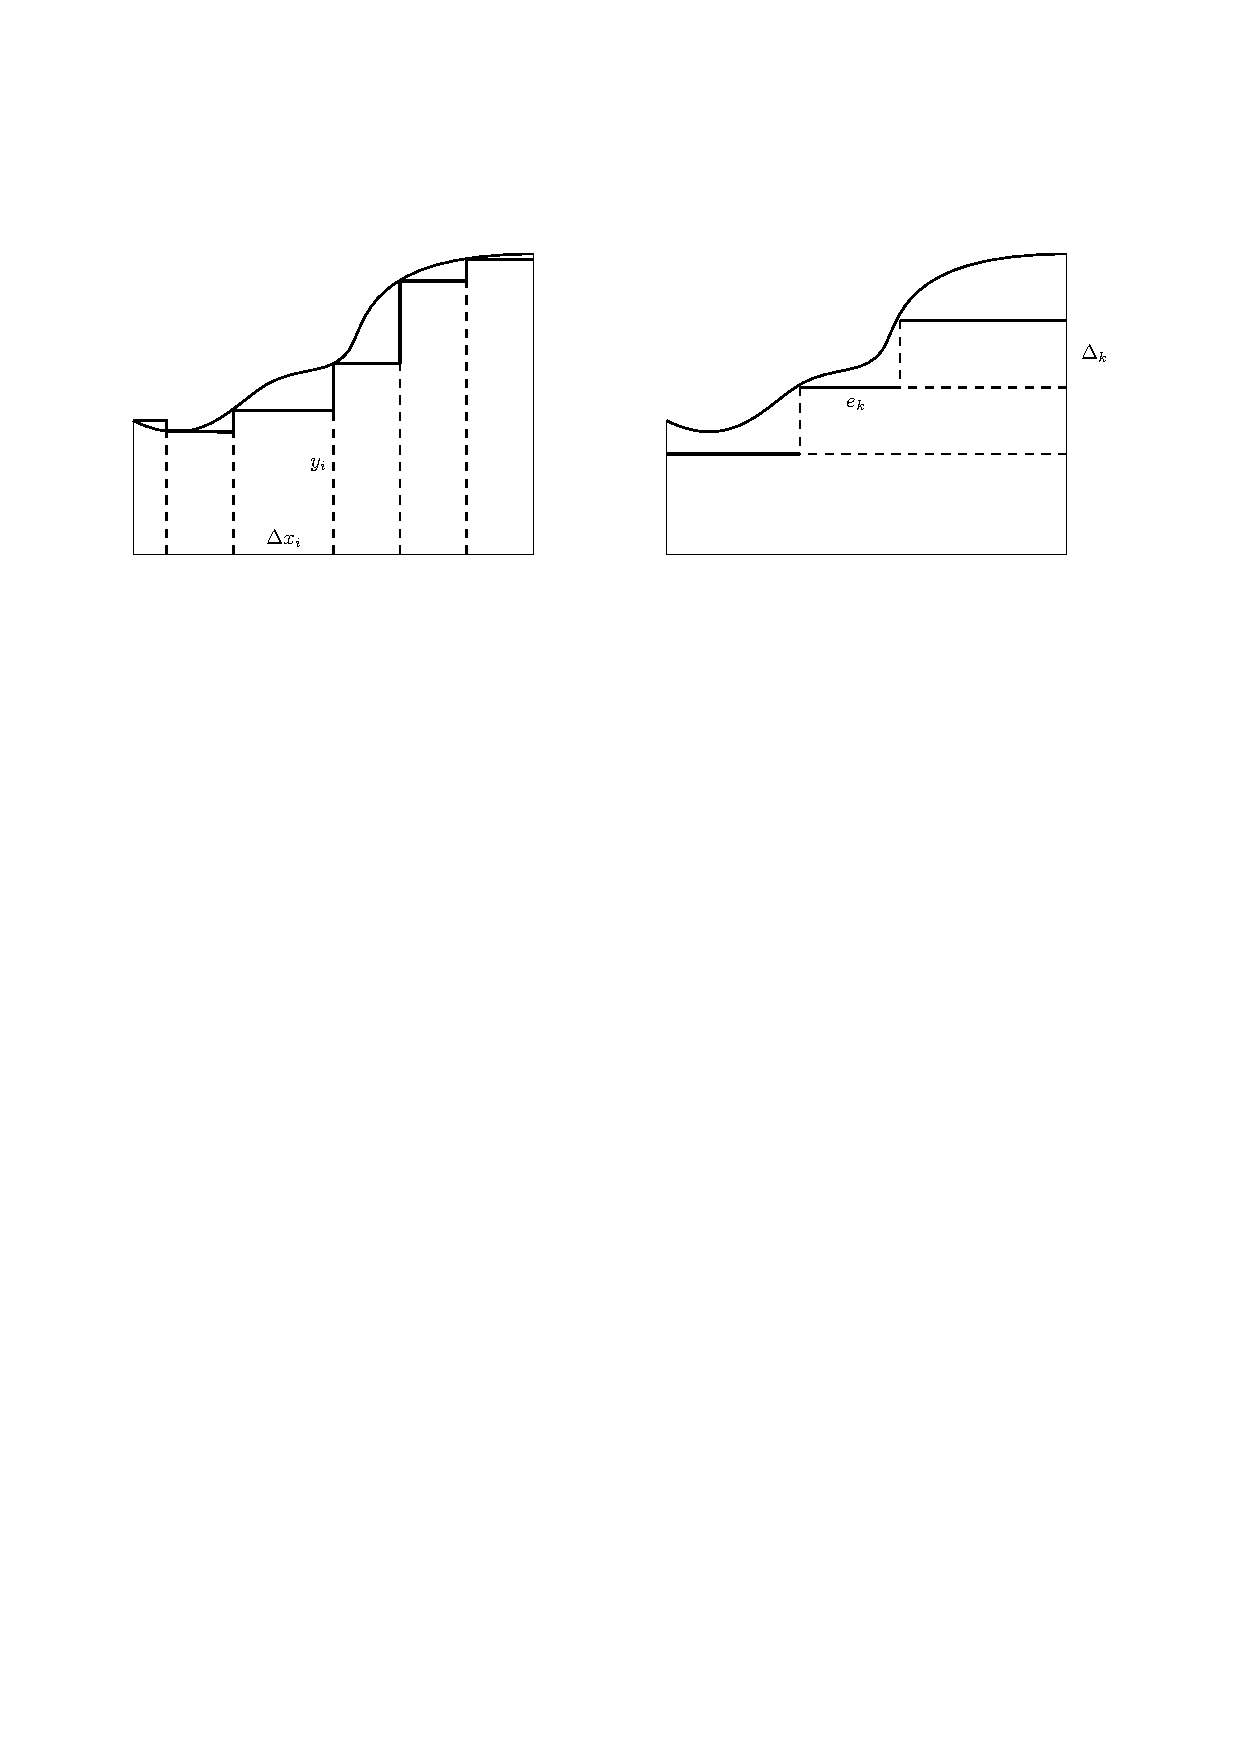
\includegraphics[scale=1]{meas/lebegriman}
\end{center}
\caption{Интегралы Римана и Лебега}
\label{fig:meas::rimleb}
\end{figure}


\paragraph{Сравнение несобственного интеграла и интеграла Лебега}
\label{par:meas::impleb}

\begin{thrm}\label{thrm:meas::impleb}
  Пусть $f \geqslant 0 \lor f \in \summb\bigl([a;b\bigr),\lambda)$. Тогда
  $\displaystyle \int_{[a;b)} f \, \del \lambda = \int _a ^{\to b} f$.
\end{thrm}
\begin{tproof}
  Cвести к собственному, а дальше непрерывность меры.
  Реально, все уже  доказано в \ref{thrm:meas::contint} и \ref{prop:meas::meas::bcont}
\end{tproof}

Поведение становится разным на не суммируемых функициях.
Например, $\dint_0^\infty \frac{\sin x}{x}$ сходится, но не абсолютно.
Значит, аналогичный лебеговский интеграл не суммируется.

\paragraph{Интеграл по дискретной мере и мере, задаваемой плотностью}
\label{par:meas::discint}

\begin{thrm}\label{thrm:meas::discint::mol}
  Пусть $\mu = \sum_{k} m_k \delta_{a_k}$, $\{a_k\} \in X$ и  $f\colon X \to \R$, 
  $f \geqslant 0$ или $f\in \summb (X,\mu)$.
  Тогда \[
    \int_X f \, \del \mu = \sum_{k} f(a_k) \cdot \underbrace{m_k}_{\mu \{a_k\}}
  \]
\end{thrm}

\begin{tproof}
  Счётная аддитивность интеграла поможет(\ref{thrm:meas::infadd})
  А на одноточечном множестве любая функция простая.
\end{tproof}


\begin{exmp}\label{exmp:meas::discint::series}
  Пусть $\mu A=\#A$. Тогда \[
    \sum_{m,n\in\N} = \int _{\N^2} f(m,n) \, \del \mu
  \]
  Причем условия сходимости  
  ряда такие же, как у интеграла Лебега: 
  \[
    \left[\;
    \begin{aligned}
      \forall\, m,n\in \N \holds a_{m,n} &\geqslant 0 \\
      \sum_{m,n\in\N} |a_{m,n}| &< \infty \\
    \end{aligned} \right.
  \]
\end{exmp}


\begin{defn}\label{defn:meas::discint::dens}
  Пусть задана пара \note{тройка, но все же поняли, что сигма-алгебра имелась в виду} 
  $(X, \mu)$, $\rho \colon X \to \R$, измерима, $\rho \geqslant 0$. 
  Тогда 
  \begin{itemize}
    \item $\displaystyle \nu(E) := \int_E \rho \, \del \mu $~--- мера, задаваемая плотностью
      $\rho$
    \item $\rho$~--- плотность меры $\nu$ относительно меры $\mu$.
  \end{itemize}
\end{defn}

\begin{rem*}
  Она правда мера, интеграл счётно-аддитивен.
\end{rem*}

\begin{thrm}\label{thrm:meas::discint::intchg}
  Пусть выполнены <<обычные>> условия на $f$. Тогда 
  $\displaystyle \int_X f \, \del \nu = \int_X f \rho \, \del \mu$.
\end{thrm}
\begin{tproof}
  Сначала разберёмся с простыми функциями. \[
    \int_X g \, \del \nu =  \sum_k c_k \nu (E_k)
    = \sum_k \int_X c_k \rho \cdot \ind_{E_k}\, \del \mu
    = \int_X \left(\sum_k c_k \cdot \ind_{E_k}\right)\, \rho \, \del \mu
    = \int_X f \rho \, \del \mu 
  \]
  Для неотрицательных поможет теорема Леви (\ref{thrm:meas::levi}), 
  а с суммируемыми уже всё просто.
\end{tproof}

\paragraph{Мера Лебега-Стилтьеса. Интеграл по распределению}
\label{par:meas::lebstil}

\begin{defn}\label{defn:meas::lebstil::meas}
  Пусть $I \subset \R$, $F \colon I \to \R$, $F \nearrow$, $F(x) = F(x-0)$ 
  (непрерывна слева).\note{А можно и без. Тогда $\nu([a;b)) = F(b-0) - F(a-0)$,
  см.~\ref{makpodk}}.

  Рассмотрим порождённую полуинтервалами $[a;b) \subset I$ алгебру.
  По сути, $\Cell_1$.
  Введём <<объём>> $\nu_F \colon \nu([a;b)) = F(b) - F(a)$.
  
  Тогда мера Лебега-Стилтьеса $\mu_F$~--- стандартное продолжение $\nu_F$ на некоторую
  $\sigma$-алгебру $\mathcal M_F$.
\end{defn}

\begin{rem}
  Здесь надо доказывать \emph{счётную} аддитивность, а то как продолжать $\nu$, если она~--- не
  мера?

  Делается это аналогично аддитивности обычного объёма, тоже надо покрывать открытыми 
  множествами ячейки из объединения. См~\ref{thrm:meas::ledeg::infadd}
\end{rem}
\begin{rem}
  $\sigma$-конечность~--- очевидна.
\end{rem}
\begin{rem}
  При таком задании объёма непрерывность $g$ слева жизненно необходима. Иначе нету непрерывности
  меры.
\end{rem}



\subparagraph{Свойства мемы Лебега-Стилтьеса}

\begin{prop}\label{prop:meas::lebstil::clos}
  Пусть $\Delta = [a;b]$. Тогда $\mu \Delta  = F(b+0) - F(a)$.
\end{prop}

\begin{prop}\label{prop:meas::lebstil::point}
  Пусть $\Delta = \{a\}$. Тогда $\mu \Delta  = F(a+0) - F(a)$.
\end{prop}

\begin{prop}\label{prop:meas::lebstil::open}
  Пусть $\Delta = (a;b)$. Тогда $\mu \Delta  = F(b) - F(a+0)$.
\end{prop}

Доказывается всё это из непрерывности $\mu_F$.

\begin{lem}\label{lem:meas::lebstil::smoothF}
  Пусть $F \in C(I)$, $\Delta \subset I$.
  Тогда $\mu_F (\Delta) = \dint_\Delta F'(t) \, \del \lambda$.
\end{lem}
\begin{lproof}
  Мы в~\ref{thrm:meas::contint} уже доказывали, что для непрерывных функций интеграл по мере
  совпадает с интегралом Ньютона-Лейбница. 
\end{lproof}
\begin{rem}\label{rem:meas::lebstil::smoothF}
  Еще можно сказать, что $F$ задана плотностью $\rho = F'$.
\end{rem}

\begin{thrm}\label{thrm:meas::lebstil::int}
  Пусть $F\nearrow$, кусочно-гладка на $I \subset \R$, а для $f$ выполнены обычные
  условия ($X = \borel$, $\mu = \mu_F$). Промежутки гладкости $F$ обозначим за $(c_k, c_{k+1})$.
  Тогда 
  \[
    \int_X f\, \del \mu_F = \sum_k \int_{c_k}^{c_{k+1}} f F' \, \del \lambda +
\sum_k f(c_k) \, \underbrace{\Delta_{c_k} F}_{\mathclap{\text{скачок в $c_k$}}}
  \]
\end{thrm}
\begin{tproof}
  По счётной аддитивности разобъем на непрерывные куски и точки. 

  Для точек:\ref{prop:meas::lebstil::point}

  Для непрерывных  кусков поможет интеграл по мере, заданной плотностью.
  См~\ref{thrm:meas::discint::intchg} 
\end{tproof}

\begin{defn}[Образ мемы]\label{defn:meas::lebstil::imag}
  Пусть $(X,\alg,\mu)$~--- пространство с мемой, $f\colon X \to Y$. 
  Превратим и $Y$ в пространство с мемой.
  \begin{enumerate}
    \item $\alg' = \{E \subset Y \mid f^{-1} (E) \in \alg\}$.
    \item $\mu' \equiv \nu = \mu \circ f^{-1} $.
  \end{enumerate}
\end{defn}
Корректность докажется из свойств прообраза.

\begin{thrm}\label{thrm:meas::lebstil::imfun}
  Пусть для $g\colon Y \to \R$ выполнены обычные условия ($\alg = \alg'$, $\mu=\nu$).
  Тогда $\displaystyle \int_Y g \, \del \nu  = \int_X (g \circ f)\, \del \mu$.
\end{thrm}
\begin{tproof}
  Пусть $g$~--- простая. 
  \[
    \int_Y g\, \del \nu = \sum_k c_k \nu (E_k) = \sum_k c_k \mu \bigl(f^{-1} (E_k)\bigr)
  \]
  С другой стороны \[
    g(f(x)) = c_k \Leftrightarrow f(x) \in E_k \Leftrightarrow x \in f^{-1}(E_k) 
    \: \Longrightarrow \:
    g \circ f = \sum_k c_k \cdot \ind_{f^{-1}(E_k)}
  \]
  А дальше~--- как обычно, через теорему Леви (\ref{thrm:meas::levi}).
\end{tproof}

\begin{defn}[Функция распределения]\label{defn:meas::lebstil::distr}
  Пусть задано $(X, \mu)$, $\mu X < + \infty$, $f\colon X \to \R$. Тогда
  $F(t) := \mu X  [f <t]$. Как видно, она возрастает и непрерывна слева.
\end{defn}

\begin{thrm}\label{thrm:meas::lebstil::distint}
  Пусть задано $(X, \mu)$, $\mu X < + \infty$, выполнены обычные условия для $f$.
  Тогда $\displaystyle \int_X f \, \del \mu = \intR t \, \del \mu_F$.
\end{thrm}
\begin{tproof}
  Следствие~\ref{thrm:meas::lebstil::imfun} при  $g(t) = t$, $\nu = \mu_F$~--- мера Лебега-Стилтъеса
  порожденная функцией распределения $F(t)$.
\end{tproof}

\paragraph{Интеграл Эйлера-Пуассона}
\label{par:meas::eulpuass}

\begin{prop}\label{prop:meas::eulpuass}
  $\displaystyle \int_{\R^2} e^{-(x^2 + y^2)}\, \del \lambda_2 = \pi $ 
\end{prop}

\begin{lproof}
  Проще рассматривать $g(x,y) = -e^{ -(x^2 + y^2) }$. Тогда
  \[
    \begin{split}
      F(t) &= \mu \R^2 [g(x,y) < t] =^* \mu \{x,y \mid -(x^2 + y^2) > \ln(-t) \} =\\
           &= \mu \{ x,y \mid x^2 + y^2 < -\ln(-t) \} =^* 
        \begin{cases}
          -\pi \ln(-t), & -1 \leqslant t < 0 \\
          0,            & t < -1             \\
          \infty ,      & t \geqslant 0
        \end{cases}
      \end{split}  
  \]
  (${}^*$ посередине не стали тащить все варианты)

  Здесь происходит некоторая магия. Можно как-то помахать руками и выкинуть всё, кроме
  $[-1;0)$.
  
  С частью больше нуля вообще ничего не понятно. Единственный вариант~---
  понимать здесь интеграл как предел конечного, по расширяющимся окружностям. В таком случае,
  после какого-то $t$ $F= \rm const$. Тогда и производная там ноль. Так что будем считать, что
  $F = \infty \Leftrightarrow F = \rm const$.
  
  Применять теорему \ref{thrm:meas::lebstil::distint} 
  здесь тоже некорректно, но для ограниченных областей можно было бы.

  \[
    \int_{\R^2} f\, \del \lambda_2  = \int_{- \infty }^ \infty  t \, \del \mu_F (t)
    = \int_{-1}^0 t F'(t) 
    = \pi \int_{-1}^0 t  \cdot \left(- \frac 1 {-t} \cdot (-1) \right) \, \del t = -\pi 
  \]
\end{lproof}



\paragraph{Вероятностный смысл мемы}
\label{par:meas::prob}

\plholdev{Табличка с соответствием}

\paragraph{Геометрический смысл меры Лебега. Принцип Кавальери}
\label{par:meas::geomleb}

\begin{defn}\label{defn:meas::geomleb::proj}
  Пусть $E \subset \R^m \times \R^n \in \lebesgue_{m+n}$.
  \begin{itemize}[$\triangleright$]
    \item $E_x      = \{ y\in \R^n \mid (x,y) \in E\}$~--- <<срез>>
    \item $\Pi_1(E) = \{ x\in \R^m \mid E_x \neq \varnothing\}$~--- <<проекция>>
  \end{itemize}
\end{defn}

\begin{exmp}\label{exmp:meas::geomleb::planarproj}
  См картинку~\ref{fig:meas::geomleb::proj}

  \begin{figure}
  \begin{center}
    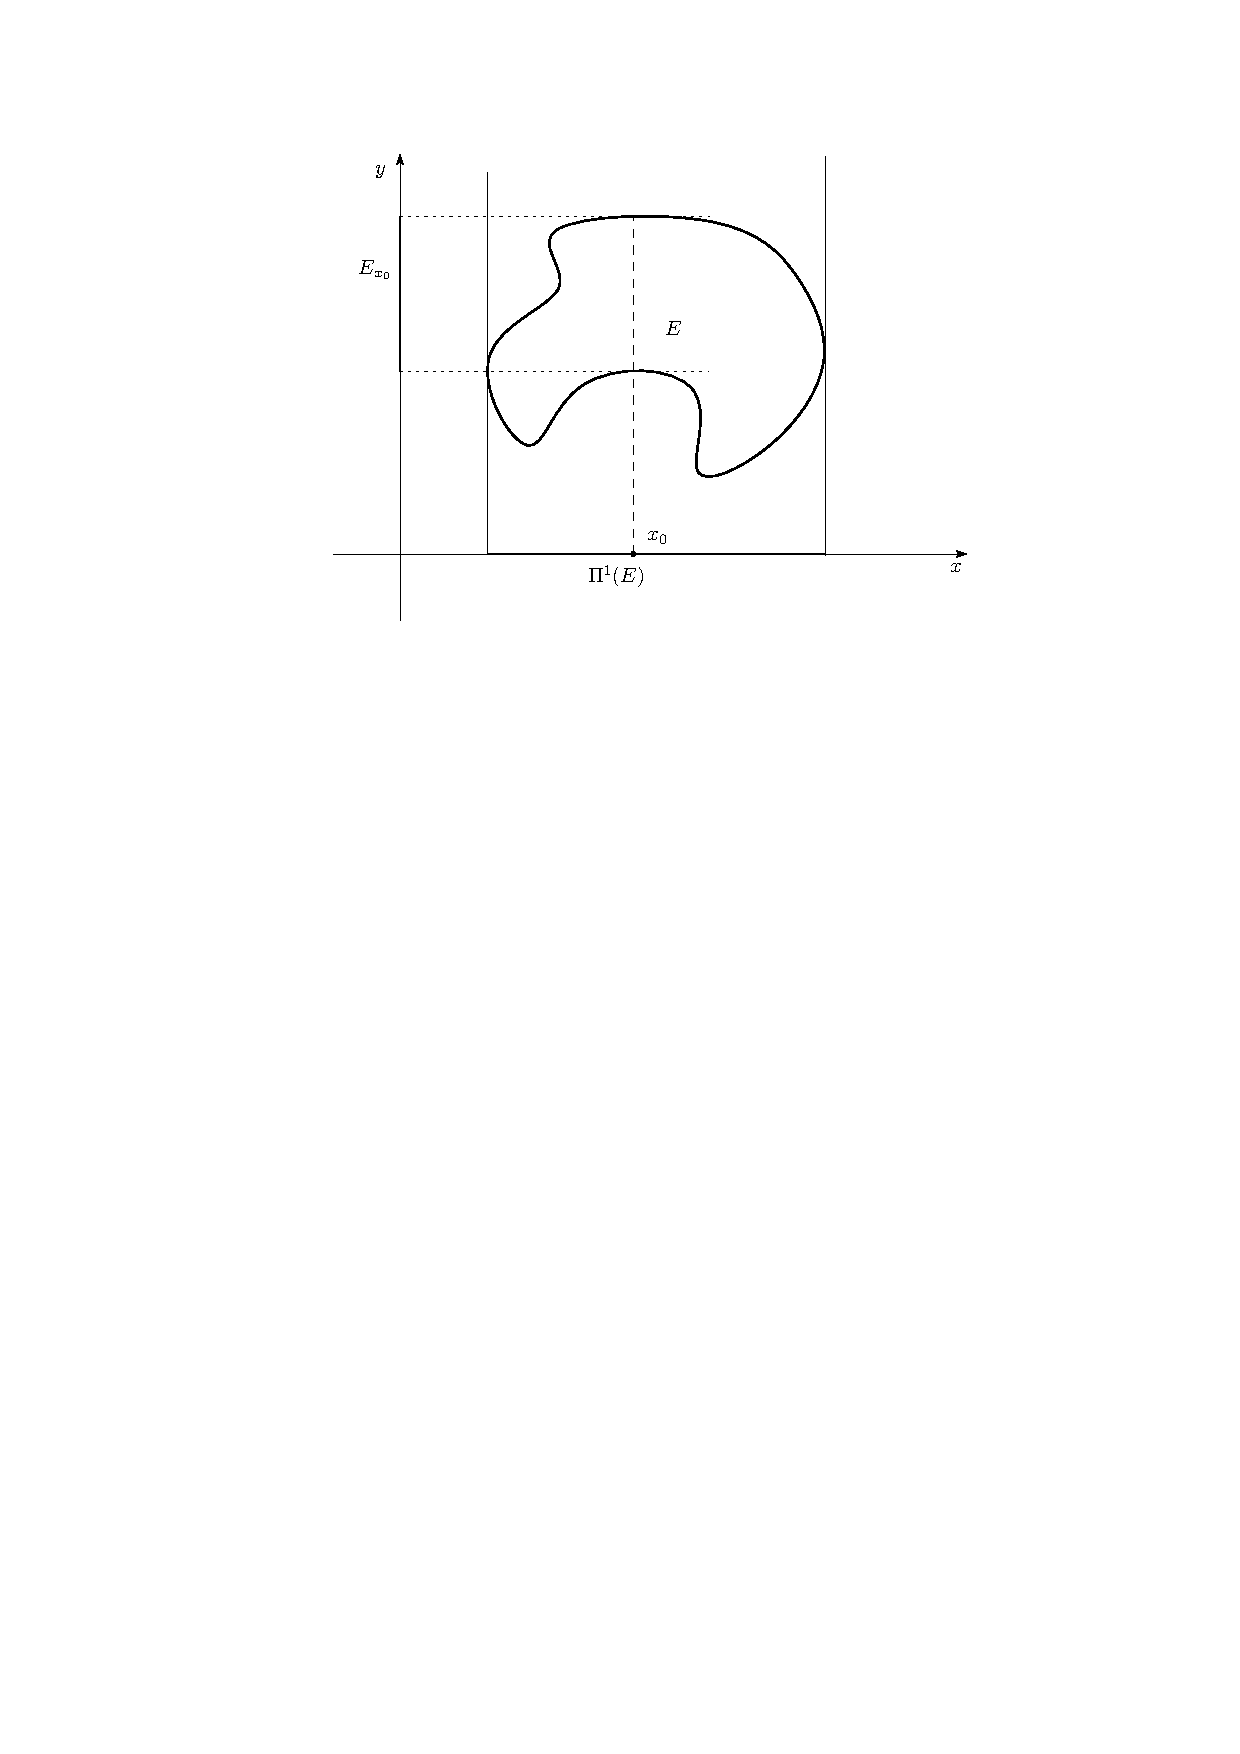
\includegraphics[scale=1]{meas/proj}
  \end{center}
  \caption{Проекции и срезы для двумерья}
  \label{fig:meas::geomleb::proj}
  \end{figure}
  
\end{exmp}

\begin{thrm}\label{thrm:meas::geomleb::cav}
  Пусть $E \in \lebesgue_{m+n}$, $E_x \in \lebesgue_{n} \alev x$,
  $\varphi(x) = \lambda_n(E_x)$ измерима относительно $\lebesgue_{m}$.

  Тогда 
  \[
    \lambda_{m+n} (E) = \int_{\R^m} \lambda_n (E_x) \, \del \lambda_m
  \]
\end{thrm}
\begin{tproof}
  \begin{enumerate}
    \item $E = \displaystyle \prod_{k=1}^\infty \Delta^k$\\
      Здесь просто $E = E_1 \times E_2$, так что
      \[
        E_x = \begin{cases}
          E_2, & x \in E_1 \\
          0, & x \not\in E_1 \\
        \end{cases} \; \Rightarrow \;
        \lambda_n  E_x = \begin{cases}
          \lambda_n E_2, & x \in E_1 \\
          0, & x \not\in E_1 \\
        \end{cases} 
      \]
      Отсюда \[
        \int_{\R^m} \lambda_n E_x \, \del \lambda_m = \int_{E_1} \lambda_n E_x \, \del \lambda_m 
        = \lambda_m (E_1) \cdot \lambda_n(E_2) = \lambda_{m+n} (E)
      \]
    \item $E = \displaystyle \bigsqcup_{k=1}^\infty E_k$, $E_k$~--- ячейка\\
      Здесь $\lambda_n E_x = \sum_k \lambda_n (E_k)_x$, а дальше теорема
      Леви для рядов~\ref{lem:meas::almev::blseries}
    \item $E \in G_\delta \Leftrightarrow G = \bigcap_k G_k$, $G_k \in \open$, причём 
      $G_1 \supset G_2 \supset \cdots$. \\
      Здесь уже нужна теорема Леви <<вверх ногами>> \ref{lem:meas::almev::blov}
    \item $E$ измеримо и ограничено. \\
      Из регулярности меры Лебега (точнее, из следствия~\ref{cor:meas::ledeg::gdelta}
      к ней)
      $\exists\, A\in G_\delta \that A = E \cup N$, а $\lambda(N) = 0$.
    \item Для неограниченных~--- представить через объединение ограниченных.
      Мера Лебега ведь сигма-конечна.
  \end{enumerate}
\end{tproof}

\begin{defn}[График]\label{defn:meas::geomleb::plot}
  $\Gamma^f = \{ (x,t) \in \R^{n+1} \mid t = f(x)\}$.
\end{defn}
\begin{defn}[Подграфик]\label{defn:meas::geomleb::subplot}
  $\Gamma_-^f = \{ (x,t) \in \R^{n+1} \mid 0 \leqslant t \leqslant f(x)\}$.
\end{defn}
\begin{defn}[Надграфик]\label{defn:meas::geomleb::supplot}
  $\Gamma_+^f = \{ (x,t) \in \R^{n+1} \mid t \geqslant f(x)\}$.
\end{defn}
Для знакопеременных можно модуль навесить, но редко встречалось.

\begin{lem}\label{lem:meas::geomleb::plotmeas}
  $\lambda_{n+1} \Gamma^f = 0$.
\end{lem}
\begin{thrm}[Геометрический смысл интеграла]\label{thrm:meas::geomleb::geomsense}
  Пусть $f\colon \R^n \to \R$, измерима, $ \geqslant 0$. Тогда
  \begin{enumerate}
    \item $\Gamma_-^f$ измеримо по $\lambda_{n+1}$
    \item $\lambda_{n+1}\Gamma_-^f = \int_{\R^n} f\, \del \lambda_n$.
  \end{enumerate}
\end{thrm}
\begin{tproof}
  \begin{enumerate}
    \item Для индикатора второе утверждение теоремы очевидно. А вот с первым всё хуже.

      В принципе, это следует вроде следует из того, что алгебра 
      $\Cell_k \times [0;1]$ порождает $\Cell_{k+1}$, но \quest.

    \item Для простых тоже всё очевидно, объединение измеримых~--- измеримо.
    \item Для неотрицательных~--- через теорему Леви  для рядов (\ref{lem:meas::almev::blseries}).
      Предел измеримых~--- измерим.
  \end{enumerate}
\end{tproof}

\paragraph{Сведение кратного интеграла к повторному}
\label{par:meas::mult}

Будем в дальнейшем обозначать интегрирование по мере через $\del x$ (ну или
$\del y$), размерность определяется из размерности $x$. Еще обозначим $\del (x,y)$ через
$\del x\del y$. 

\begin{thrm}[Тонелли]\label{thrm:meas::mult::tonn}
  Пусть $f\colon \R^{m+n} \to \R$, измерима, $ \geqslant 0$, $x\in \R^m$, $y \in \R^n$.
  Тогда
  \[
    \iint_{\R^m \times \R^n} f(x,y) \, \del x\del y 
    = \int_{\R^m} \del x \int_{\R^n} f(x,y) \, \del y
  \]
\end{thrm}
\begin{tproof}
  Следствие~\ref{thrm:meas::geomleb::geomsense}. Правда снова сложности с измеримостью.
\end{tproof}

\begin{thrm}[Фубини]\label{thrm:meas::mult::fub}
  Пусть $f\colon \R^{m+n} \to \R$, измерима, $\in \summb(\R^{n+m}, \lambda_{m+n})$,
  $x\in \R^m$, $y \in \R^n$. Тогда
  \[
    \iint_{\R^m \times \R^n} f(x,y) \, \del x\del y 
    = \int_{\R^m} \del x \int_{\R^n} f(x,y) \, \del y
  \]
\end{thrm}

\paragraph{Мера Лебега и аффинные преобразования}
\label{par:meas::aff}

Главные герои этого параграфа:

\begin{itemize}[$\bigcirc$]
  \item Сдвиг: $T \colon \R^n \to \R^n$, $Tx = x+a$, $a\in \R^n$.
  \item Поворот с растяжением: $L \colon \R^n \to \R^n$, $L$~--- линейный император.
\end{itemize}


\begin{stat}\label{stat:meas::aff::shiftmeas}
  $E \in \lebesgue \Rightarrow T(E) \in \lebesgue$. 
\end{stat}
\begin{lproof}
  Для открытых всё очевидно: $f(G) \in \open$, раз это гомеоморфизм. 
  Пересечение образов~--- образ пересечения. Так что и для $G_\delta$ всё работает.

  Дальше можно вспомнить, что измеримое $E= G_\delta \cap N$, $\lambda N = 0$.
  Если множество нулевой меры, то можно покрыть его ячейками так, что 
  $\sum_k \lambda\Delta_k < \varepsilon$. Это просто из определения внешней меры.

  Поскольку размеры ячеек просто сохраняются, образ тоже будет нулевой меры.
  $N \subset \bigcup_k \Delta_k \Rightarrow f(N) \bigcup_k f(\Delta_k)$, так как объединение
  образов = образу объединения.
\end{lproof}
\begin{stat}\label{stat:meas::aff::linmeas}
  $E \in \lebesgue \Rightarrow L(E) \in \lebesgue$. 
\end{stat}
\begin{lproof}
  В случае $\det L = 0$ размерность образа меньше $n \Rightarrow $ мера равна нулю.

  Иначе, все очти аналогично рассуждению выше, только оценка меры образа сложнее.
  Пусть $\lambda \Delta = \delta ^n$, тогда
  \[
    \forall\, x, y \in \Delta \holds \|Lx - Ly\| \leqslant \|L\|\, \|x - y\| 
    \leqslant \sqrt{n} \delta \|L\|
  \]
  А значит можно уменьшая $\delta$ получить сколь угодно малые покрытия образа нуль-множества.
\end{lproof}


\begin{stat}\label{stat:meas::aff::disturb}
  Пусть $L \colon \R^n \to \R$, линейно. Тогда 
  \[
    \exists\, C \geqslant 0 \that \forall\, E \in \lebesgue \holds \lambda L(E) = C \lambda E
  \]
\end{stat}
\begin{lproof}
  Здесь можно разобраться с ячейкой $[0;1)^n$, а дальше обычными способами построить весь мир 
  из ячеек.
\end{lproof}

\begin{thrm}\label{thrm:meas::aff::deter}
  $C$ из прошлой теоремы равно $\bigl|\det [L]\bigr|$.
\end{thrm}
\begin{tproof}
  тут декомпозиция на ортогональный и диагональные операторы:
  \[
    L = U_1 \, D \, U_2
  \]
  Определитель матрицы всего оператора равен определителю диагонального. Для ячеек очевидно, что
  $C = |\det D|$, ортогональный сохраняет объёмы ячеек. А дальше как обычно.
\end{tproof}
\paragraph{Мера образа при гладком отображении}
\label{par:meas::smoothimgmeas}

{\denot $J_F(x) \equiv \det F'(x)$}

\begin{thrm}\label{thrm:meas::smoothimgmeas}
  Пусть $E \in \lebesgue$, $F \colon G \subset \R^n \to \R^n$, гладкая биекция.
  Тогда $F(E) \in \lebesgue$ и $\lambda F(E) = \dint_E |\det F'(x) |\del x$.
\end{thrm}
\begin{tproof}
  \sour\underdev
\end{tproof}
\begin{tproof}
  Что делать здесь с измеримостью не очень понятно. Если с компактами ещё как-то разобраться можно,
  то вот что делать с неограниченными совсем непонятно.

  Можно поразмахивать линеаризацией и сказать, что 
  \[
    F(x) \approx F(x_k) + F'(x_k) (x-x_k)
  \]
  а последнее уже аффинное, для которых якобы что-то доказали.
\quest
\end{tproof}

\paragraph{Глакая замена переменной в интеграле}
\label{par:meas::smoothvarch}

\begin{thrm}\label{thrm:meas::smoothvarch}
  Пусть $F \colon G \subset \R^n \to R^n$, гладкая биекция.
  Пусть к тому же $E \subset F(G) \in \lebesgue$, $f\colon E \to \R$ с обычными условиями.

  Тогда\[
    \int_E f(y) \, \del y = \int_{F^{-1}(E)} f(F(x)) \cdot| J_F(x) | \, \del x
  \]
\end{thrm}
\begin{tproof}
  Хотелось бы свести это к чему-то старому, но не получится: мера не поменялась, а поменялось
  множество и функция.

  Так что надо снова доказывать для простых. Пусть
  \[
    f(y) = \sum_i c_i \cdot \ind_{B_i}(y)
  \]
  Тогда $f(y) = c_i \Leftrightarrow y = F(x) \in B_i \Leftrightarrow x\in F^{-1}(B_i) = A_i$
  Так что 
  \[
    f(y) = \sum_i c_i \cdot \ind_{A_i}(x)
  \]
  Отсюда\[
    \int_E f(y) \, \del y = \sum_i c_i \int_{A_i} |J_F(x)|\, \del x 
    = \sum_i c_i \int_{F^{-1}(E)} |J_F(x)|\cdot \ind_{A_i} \del x
    = \int_{F^{-1}(E)} f(F(x)) \cdot|J_F(x)| \,\del x
  \]
\end{tproof}

\begin{exmp}[Полярные координаты]\label{exmp:meas::smoothvarch::polar}
  \underdev
  $|J| = r$
\end{exmp}

\begin{exmp}[Сферические координаты]\label{exmp:meas::smoothvarch::sph}
  \underdev
  $|J| = r^2 \cos \psi $
\end{exmp}

\paragraph{Предельный переход под знаком интеграла}
\label{par:meas::limint}

\begin{defn}[Всякие сходимости]\label{defn:meas::limint::conv}
  Пусть $(f_n) \colon X \to \R$, $f \colon X \to \R$, $\mu$~--- мера на $X$.
  \begin{align*}
    & f_n \to f       & &:= & &\forall\, x \in X \holds f_n(x) \to f(x)      \\
    & f_n \unito^X f  & &:= & &\rho(f_n, f) = \sup\limits_X |f_n-f| \to 0     \\
    & f_n \to f \alev & &:= &&\exists\, N \subset X \colon \mu(N) = 0 
    \that \forall\, x\in X \setminus N \holds f_n(x) \to f(x).            \\
    & f_n \to^\mu f & &:= &&\forall\, \sigma > 0 \holds \mu X [ |f_n - f| \geqslant \sigma ]\to 0
    \end{align*}
\end{defn}

\begin{rem}\label{rem:meas::limint::convseq}
  $ f \unito^X f \Rightarrow f_n \to f \Rightarrow f_n \to f \alev$.
\end{rem}
\begin{rem}\label{rem:meas::limint::convmeas}
  Пусть $\mu X < \infty $, тогда
  $ f_n \to f \alev \Rightarrow f_n \to^\mu f$.
\end{rem}

\begin{rem}[Теорема Рисса]\label{rem:meas::limint::convpv}
  $ f_n \to^\mu  f \alev \Rightarrow \exists\, (n_k) \that f_{n_k} \to f \alev $.
\end{rem}

\begin{thrm}\label{thrm:meas::limint::uniint}
  $f_n \unito^X f, \mu X < \infty \Rightarrow \dint_X f_n \, \del \mu \to \int _X f$
\end{thrm}
\begin{tproof}
  \[
    \begin{split}
      \left| \int_X f_n \, \del \mu - \int_X f\, \del \mu  \right| 
      &= \left| \int_X f_n - f\, \del \mu  \right| 
      \leqslant \int_X |f_n - f| \, \del \mu 
      \leqslant \int \rho (f_n, f) \, \del \mu \\
      &= \rho (f_n ,f) \, \mu X \xto{n\to \infty} 0
    \end{split}
  \]
\end{tproof}

\begin{thrm}
  см теорему Беппо-Леви (\ref{thrm:meas::levi}) или её вариацию \ref{lem:meas::almev::blov}.
\end{thrm}

\begin{thrm}[Фату]\label{thrm:meas::limint::fatu}
  Пусть заданы $(X,\mu)$, $f_n \geqslant 0$, измеримы. Тогда
  \[
    \int_X \varliminf f_n \, \del \mu \leqslant \varliminf \int_X f_n \, \del \mu 
  \]
\end{thrm}
\begin{exmp}\label{exmp:meas::limint::gaussian}
  Ползущая на бесконечность гауссиана.
\end{exmp}
\begin{tproof}
  \[
    \varliminf f_n(x)  = \lim_{n\to \infty} \inf_{m \geqslant n} f_m (x) ; \quad 
    g_n(x) = \inf_{m \geqslant n} f_m (x) 
  \]
  Эта последовательность возрастает, мы каждый раз берем все меньше функций. 
  Так что по теореме Леви (\ref{thrm:meas::levi}) 
  \[
    \int g_n \to \int \varliminf f_n 
  \]
  Из определения инфимума $f_n \geqslant g_n$. Значит
  \[
    \varliminf \int f_n \geqslant \varliminf \int g_n = \lim \int g_n = 
    \int \varliminf f_n
  \]
\end{tproof}

\paragraph{Теорема Лебега об ограниченной сходимости}
\label{par:meas::bndconv}

\begin{thrm}\label{thrm:meas::bndconv}
  Пусть снова заданы $(X,\mu)$, $(f_n)$ измерима, $f_n \to f \alev$. К тому же
  \[
    \exists\, \varphi \in \summb \that \forall\, n \holds |f_n|  \leqslant |\varphi|
  \]
  Тогда
  \[
    \lim_{n\to \infty} \int _X f_n \, \del \mu = \int_X f\, \del \mu 
  \]
\end{thrm}
\begin{tproof}
  $f$ суммируема из теоремы Фату~\ref{thrm:meas::limint::fatu}

  Коль скоро $\varphi - f_n \geqslant 0$, 
  \[
    \int (\varphi - f)  =  \int \varliminf (\varphi - f_n) \leqslant 
    \int \varphi + \varliminf \left(- \int f_n \right) = \int \varphi - \varlimsup \int f_n
  \]
  Используя свойства верхних и нижних пределов и теорему Фату (\ref{thrm:meas::limint::fatu})
  получим 
  \[
    \int f \leqslant \varliminf \int f_n \leqslant \varlimsup \int f_n \leqslant \int f
  \]
\end{tproof}

{\denot $(\mathcal L)$~--- условия теоремы Лебега об ограниченной сходимости.}

\begin{cor}
  Пусть $f\colon T \times X \to \R$, $T \subset \R^k$, $f_t \xto{t\to t_0}{} f \alev$,
  и \[
    \exists\, V(t^0), \varphi \in \summb \that \forall\, t \in \punct V \cap T
    \holds |f_t| \leqslant |\varphi| 
  \]
  Тогда
  \[
    \int _X f_t \, \del \mu \xto{t\to t_0}{} \int_X f\, \del \mu 
  \] 
\end{cor}
\begin{lproof}
  Предел по Гейне.
\end{lproof}

{\denot $(\mathcal L_{\rm loc})$~--- условия локальной теормемы Лебега об ограниченной сходимости.}

\begin{cor}
  Непрерывность интеграла по параметру при выполнении $(\mathcal L_{\rm loc})$ и 
  непрерывности $f_t$.
\end{cor}

\paragraph*{Интеграл по меме с параметром}

Здесь часто придётся подчёркивать, что является параметром, а что~--- определяет функцию
В таких случаях параметр будет записан, как индекс

\begin{defn}[Собственный интеграл с параметром]\label{defn:meas::paruniconv::prop}
  Пусть $f\colon X \times T \to \R$, $f_t(x)\in \summb([a,b],\mu) \; \forall\, t \in T$. 
  Тогда, 
  \[
    I(t) = \int_a^{b} f(x,t) \, \del x 
  \]
  Мы здесь определяем некоторую функцию от $t$, как видно $\dom_I = T$.
\end{defn}

По идее, надо здесь переформулировать все-все-все утверждения про последовательности функций.
Надо бы узнать, что с этим делать.
\flame 
У нас в конспекте этот кусок почему-то написан про несобственные интегралы, но всюду полагается
$(\mathcal L_{\rm loc})$. Так что по сути они~--- просто интегралы по меме.

Здесь тоже есть непрерывность, дифференциируемость и интегрирование по параметру, но
все тривиально\note{ну..} следует из \ref{thrm:meas::bndconv} и \ref{thrm:meas::mult::fub}.

\paragraph{Равномерная сходимость несобственного параметрического интеграла. Признаки}
\label{par:meas::paruniconv}


\begin{defn}[Несобственный интеграл с параметром]\label{defn:meas::paruniconv::improp}
  Пусть $f\colon X \times T \to \R$,
  $f\in \summb([a,B],\mu) \;\forall\, B <b$. Тогда,
  \[
    I(t) = \int_a^{\to b} f(x,t) \, \del x := \lim_{B\to b-0} \int_a^B f(x,t) \, \del x 
    = \lim_{B\to b-0} I^B(t)
  \]
  Предполагается, что $\forall\, t \in T$ интеграл сходится поточечно. А вот суммируемость
  никто не обещал.
\end{defn}


\begin{defn}\label{defn:meas::paruniconv::uniconv}
  Говорят, что $I^B(t) \unito^T I(t)$ (сходится равномерно относительно $t, t\in T$), если 
  \note{Никто же не любит $\varepsilon$-$\delta$-определения?}
  \[
    \sup_{t\in T} \left| \int_B^{\to b} f(x,t)\right| \xto{B\to b} 0
  \]
\end{defn}

Здесь дальше всюду предполагается поточечная сходимость интеграла $\forall\, t \in T$.

\begin{thrm}[Признак Больцано-Коши]\label{thrm:meas::paruniconv::bk}
  \[
    I^B(t) \unito^T I(t) \Leftrightarrow 
    \sup_{T} \left| \int_{B_1}^{B_2} f(x,t)\, \del x \right| \xto{B_1, B_2 \to b} 0
  \]
\end{thrm}

\begin{thrm}[Признак Вейерштрасса]\label{thrm:meas::paruniconv::wei}
  Пусть $\exists\, \varphi\in \summb([a;b))\that |f(x,t)| \leqslant \varphi (x)\; \forall\, t$.
  Тогда $I^B(t) \unito^T I(T)$.
\end{thrm}

\begin{thrm}[Признак Дирихле]\label{thrm:meas::paruniconv::dir}
  Пусть $I(t) = \dint_{a}^{\to b} f(x,t) \cdot g(x,t) \, \del x$ и
  \begin{enumerate}[a)]
    \item $f(x,t) \unito^T 0$, $f(x,t) \searrow^x$ ($x\to b-0$)
    \item $G(x,t) = \dint_a^x g(\xi, t) \, \del \xi$
      \[
        \exists\, M \colon \forall\, x \in [a;b), t\in T \that | G(x,t) | \leqslant M   
      \]
  \end{enumerate}
  Тогда $I^B(t) \unito^T I(T)$.
\end{thrm}

\begin{thrm}[Признак Абеля]\label{thrm:meas::paruniconv::abel}
  Пусть $I(t) = \dint_{a}^{\to b} f(x,t) \cdot g(x,t) \, \del x$ и
  \begin{enumerate}[a)]
    \item $\exists\, M \colon \forall\, t\in T \holds f(x,t) \leqslant M$,
      $f(x,t) \searrow^x$.
    \item 
      $\displaystyle
      \int_a^{B} g(x,t) \, \del x \unito^T_{B\to b} \int_a^{\to b} g(x,t) \, \del x 
      $
  \end{enumerate}
  Тогда $I^B(t) \unito^T I(T)$.
\end{thrm}

\paragraph{Несобственные интегралы с параметром и операции анализа над параметром \underdev}
\label{par:meas::parimpconv}

\begin{thrm}\label{thrm:meas::parimpconv::lim}
  Пусть $f(x,t) \to f(x,t_0)$ для \alev $x \in [a;b)$ и $I^B(t) \unito^{V(t^0)} I(t)$.
  \note{Это не очень докажется без конечности меры $V(t_0)$ ,а то интеграл может сходится, а
  функция не быть суммируемой}
  Тогда $I \xto{t\to t_0} I(t_0)$.
\end{thrm}

\begin{thrm}\label{thrm:meas::parimpconv::diff}
  Пусть для $\alev x \; \exists\, f_t'(x,t)$, непрерывна на $[a;b) \times \underbrace{[c;d)}_T$. 
  Допустим,
  \begin{enumerate}[a)]
    \item $I(t) = \dint_a^{\to b} f (x,t)\, \del x$ сходится $\forall\, t \in T$
    \item $\dint_a^{\to b} f_t' (x,t)\, \del x$ равномерно сходится относительно $t \in T$
  \end{enumerate}
  Тогда $\exists\, I'(t_0) = \dint_a^{\to b} f_t'(x,t_0)\, \del x$
\end{thrm}
\begin{rem*}
  Здесь нужна сходимость $I$, чтобы хоть где-то были конечные значения $I(t)$, нам их
  разность считать.
\end{rem*}

\begin{thrm}\label{thrm:meas::parimpconv::int}
  Пусть для $\alev x \; \exists\, f(x,t)$, непрерывна на $[a;b) \times \underbrace{[c;d)}_T$. 
  Допустим,
  $I(t) = \dint_a^{\to b} f (x,t)\, \del x$ равномерно сходится относительно $t \in T$
  
  Тогда \[
    \dint_c^d I(t)\, \del t = \dint_a^{\to b} \del x \int_c^d f(x,t)\, \del t
  \]
\end{thrm}


\paragraph{\texorpdfstring{$\Gamma$}{Г}-функция Эйлера}
\label{par:meas::gamma}

\begin{defn}\label{defn:meas::gamma}
  $\displaystyle \Gamma(t) = \int_0^\infty x^{t-1} e^{-x} \, \del x$
\end{defn}

\subparagraph{Свойства}

\begin{enumerate}[$1^\circ$]
  \item Определена для всех $t>0$.
  \item $\Gamma (1) = 1$
  \item $\forall\, t \Gamma (t+1) = t \Gamma (t)$
  \item $n\in \N$ $\Gamma(n+1) = n!$
  \item\label{it:meas::gamma::conc} $\Gamma$-выпукла
  \item $\Gamma \sim \frac{1}{t} $ при $t\to 0$
  \item $\Gamma(t+1) \sim \sqrt{2\pi} \sqrt{t} \cdot t^t e^{-t}$ при $t\to \infty$.
  \item $\Gamma(t) \cdot \Gamma(1-t) = \frac{\pi}{\sin \pi t}$. (формула отражения)
\end{enumerate}
\begin{lproof}
  Доказать интересно лишь \ref{it:meas::gamma::conc}
  Здесь нужно мажорировать интеграл от $n$-ой производной. Выберем окрестность $t^0$
  равную $(t_1;t_2)$, $t_1 > 0$.
  \[
    \frac{\partial^n}{\partial t^n} x^{t-1} e^{-x} = x^{t-1}\, e^{-x}\, \ln ^n (x)
  \]
  Надо разобраться с $x^{t-1}$. В $(0;1)$ можно оценить его как $x^{t_1 -1}$, $t_1$~--- фиксировано.
  Логарифм убывает медленнее $x^{-p}$, пусть $p = 1/2 \cdot t_1$. С экспонентой 
  проблем нет, её единицей оценим

  При $x>1$ оценим $x^{t-1}$ как $x^{t_2-1}$, экспонента забьёт все остальное.
  Так что $\varphi$~--- суммируемая мажоранта
  \[
    \varphi(x) = 
    \begin{cases}
      x^{\lfrac{1}{2} t_1 - 1},& 0 < x< 1 \\
      x^{t_2 - 1}\ln^n (x) \, e^{-x},& x \geqslant 1 \\
    \end{cases}
  \]
  Отсюда по следствию из \ref{thrm:meas::bndconv} производные от $\Gamma$ существуют.
  Как видно, выпуклость здесь уже совсем очевидна, подынтегральное выражение положительно.
\end{lproof}

Гамма-функцию можно продолжить на отрицательную область, через формулу отражения.
И на комплексную, там будет сходимость при $\Im z > 0$.

\paragraph{B-функция}
\label{par:meas::beta}

\begin{defn}\label{defn:meas::beta}
  $\displaystyle B(y,z) = \int_0^1 x^{y-1} (1-x)^{z-1} \, \del x$.
\end{defn}

\subparagraph{Свойства}
\begin{enumerate}[$1^\circ$]
  \item $B(y,z) = B(z,y)$.
  \item $B(y,z) = \dfrac{\Gamma(y) \Gamma(z)}{\Gamma(y+z)}$.
\end{enumerate}

\begin{lproof}
  Начнём с $\Gamma(y) = \dint_0^\infty x^{y-1} e^{-x} \, \del x$. Пусть $x=ut$, $t>0$. 
  Тогда
  \[
    \Gamma(y) = \int_0^\infty t^{y-1} u^{y-1} \, e^{-ut} \, t \, \del u 
    \Rightarrow 
    \frac{\Gamma(y)}{t^y} = \int_0^\infty u^{y-1} e^{-ut} \, \del u
  \]
  Заменим: $y \gets y+z, t \gets t+1$.
  \[
    \frac{\Gamma(y+z)}{t^{y+z}} = \int_0^\infty u^{y+z-1} e^{-ut}\, e^{-u}\, \del u
    \Rightarrow 
    \int_0^\infty \frac{\Gamma(y+z)}{(1+t)^{y+z}} \, t^{y-1} \, \del t 
    = \int_0^\infty \del t\, t^{y-1} \, \int_0^\infty u^{y+z-1} e^{-ut} e^{-u} \, \del u
  \]
  Докажем, что
  \[
    \int_0^\infty \frac{t^{y-1}}{(1+t)^{y+z}} \, \del t = B(y,z)
  \]
  Это очевидно после замены $t = \frac{1-s}{s} $.

  Разберёмся с оставшейся частью
  \[
    \begin{split}
      \int_0^\infty \del t\, t^{y-1} \, \int_0^\infty u^{y+z-1} e^{-ut} e^{-u} \, \del u
      &= \int_0^\infty\del u\, e^{-u}\,u^{y+z-1}\int_0^\infty\del t\left(e^{-ut} t^{y-1}\right) \\
      &= \int_0^\infty \del u \, u^{y+z-1} e^{-u} \, \frac{\Gamma(y)}{u^y} 
      = \Gamma(y) \Gamma (z)
    \end{split}
  \]
\end{lproof}

\paragraph{Объём \texorpdfstring{$n$}{n}-мерного шара}
\label{par:meas::ball}

\begin{thrm}\label{thrm:meas::ball}
  Пусть $B_n(R) = \{x \in \R^n \mid \|x\| \leqslant R \}$~-- $n$-мерный шар.
  Тогда 
  \[
    \lambda_n B_n(R) = \frac{\pi ^{n/2} R^n}{\tfrac{n}{2} \cdot \Gamma(\tfrac{n}{2})} 
  \]
\end{thrm}
\begin{tproof}
  Докажем всё для шара единичного радиуса, из свойств меры Лебега можно доказать для
  остальных.
  \[
    \begin{split}
      V_n 
      &= \int_{B(1)} 1 \, \del \lambda_n 
      = \int_{-1}^1 \del x_1 \, B_{n-1}\left(\sqrt[n-1]{1-x_1^2}\right)
      = V_{n-1} \int_{-1}^1 (1-x_1^2) ^{\lfrac{n-1}{2}} \, \del x_1 \\
      &= /t=x_1^2/ = 2 V_{n-1} \int _0^1 (1-t)^{\lfrac{n-1}{2}} \cdot \frac{1}{2} t^{-1/2} \, \del t
      = V_{n+1} B(\frac 1 2, \frac {n+1} 2)
    \end{split}
  \]
  Одна из двоек вылезла из-за чётности. Упрощая, используя кучу доказанного про гамма- и
  бета-функции, получим желаемое.
\end{tproof}

\end{document}
% vim: tw=100 cc=100
